% Options for packages loaded elsewhere
\PassOptionsToPackage{unicode}{hyperref}
\PassOptionsToPackage{hyphens}{url}
%
\documentclass[
  ignorenonframetext,
]{beamer}
\usepackage{pgfpages}
\setbeamertemplate{caption}[numbered]
\setbeamertemplate{caption label separator}{: }
\setbeamercolor{caption name}{fg=normal text.fg}
\beamertemplatenavigationsymbolsempty
% Prevent slide breaks in the middle of a paragraph
\widowpenalties 1 10000
\raggedbottom
\setbeamertemplate{part page}{
  \centering
  \begin{beamercolorbox}[sep=16pt,center]{part title}
    \usebeamerfont{part title}\insertpart\par
  \end{beamercolorbox}
}
\setbeamertemplate{section page}{
  \centering
  \begin{beamercolorbox}[sep=12pt,center]{part title}
    \usebeamerfont{section title}\insertsection\par
  \end{beamercolorbox}
}
\setbeamertemplate{subsection page}{
  \centering
  \begin{beamercolorbox}[sep=8pt,center]{part title}
    \usebeamerfont{subsection title}\insertsubsection\par
  \end{beamercolorbox}
}
\AtBeginPart{
  \frame{\partpage}
}
\AtBeginSection{
  \ifbibliography
  \else
    \frame{\sectionpage}
  \fi
}
\AtBeginSubsection{
  \frame{\subsectionpage}
}
\usepackage{amsmath,amssymb}
\usepackage{iftex}
\ifPDFTeX
  \usepackage[T1]{fontenc}
  \usepackage[utf8]{inputenc}
  \usepackage{textcomp} % provide euro and other symbols
\else % if luatex or xetex
  \usepackage{unicode-math} % this also loads fontspec
  \defaultfontfeatures{Scale=MatchLowercase}
  \defaultfontfeatures[\rmfamily]{Ligatures=TeX,Scale=1}
\fi
\usepackage{lmodern}
\usetheme[]{Madrid}
\ifPDFTeX\else
  % xetex/luatex font selection
\fi
% Use upquote if available, for straight quotes in verbatim environments
\IfFileExists{upquote.sty}{\usepackage{upquote}}{}
\IfFileExists{microtype.sty}{% use microtype if available
  \usepackage[]{microtype}
  \UseMicrotypeSet[protrusion]{basicmath} % disable protrusion for tt fonts
}{}
\makeatletter
\@ifundefined{KOMAClassName}{% if non-KOMA class
  \IfFileExists{parskip.sty}{%
    \usepackage{parskip}
  }{% else
    \setlength{\parindent}{0pt}
    \setlength{\parskip}{6pt plus 2pt minus 1pt}}
}{% if KOMA class
  \KOMAoptions{parskip=half}}
\makeatother
\usepackage{xcolor}
\newif\ifbibliography
\usepackage{color}
\usepackage{fancyvrb}
\newcommand{\VerbBar}{|}
\newcommand{\VERB}{\Verb[commandchars=\\\{\}]}
\DefineVerbatimEnvironment{Highlighting}{Verbatim}{commandchars=\\\{\}}
% Add ',fontsize=\small' for more characters per line
\usepackage{framed}
\definecolor{shadecolor}{RGB}{248,248,248}
\newenvironment{Shaded}{\begin{snugshade}}{\end{snugshade}}
\newcommand{\AlertTok}[1]{\textcolor[rgb]{0.94,0.16,0.16}{#1}}
\newcommand{\AnnotationTok}[1]{\textcolor[rgb]{0.56,0.35,0.01}{\textbf{\textit{#1}}}}
\newcommand{\AttributeTok}[1]{\textcolor[rgb]{0.13,0.29,0.53}{#1}}
\newcommand{\BaseNTok}[1]{\textcolor[rgb]{0.00,0.00,0.81}{#1}}
\newcommand{\BuiltInTok}[1]{#1}
\newcommand{\CharTok}[1]{\textcolor[rgb]{0.31,0.60,0.02}{#1}}
\newcommand{\CommentTok}[1]{\textcolor[rgb]{0.56,0.35,0.01}{\textit{#1}}}
\newcommand{\CommentVarTok}[1]{\textcolor[rgb]{0.56,0.35,0.01}{\textbf{\textit{#1}}}}
\newcommand{\ConstantTok}[1]{\textcolor[rgb]{0.56,0.35,0.01}{#1}}
\newcommand{\ControlFlowTok}[1]{\textcolor[rgb]{0.13,0.29,0.53}{\textbf{#1}}}
\newcommand{\DataTypeTok}[1]{\textcolor[rgb]{0.13,0.29,0.53}{#1}}
\newcommand{\DecValTok}[1]{\textcolor[rgb]{0.00,0.00,0.81}{#1}}
\newcommand{\DocumentationTok}[1]{\textcolor[rgb]{0.56,0.35,0.01}{\textbf{\textit{#1}}}}
\newcommand{\ErrorTok}[1]{\textcolor[rgb]{0.64,0.00,0.00}{\textbf{#1}}}
\newcommand{\ExtensionTok}[1]{#1}
\newcommand{\FloatTok}[1]{\textcolor[rgb]{0.00,0.00,0.81}{#1}}
\newcommand{\FunctionTok}[1]{\textcolor[rgb]{0.13,0.29,0.53}{\textbf{#1}}}
\newcommand{\ImportTok}[1]{#1}
\newcommand{\InformationTok}[1]{\textcolor[rgb]{0.56,0.35,0.01}{\textbf{\textit{#1}}}}
\newcommand{\KeywordTok}[1]{\textcolor[rgb]{0.13,0.29,0.53}{\textbf{#1}}}
\newcommand{\NormalTok}[1]{#1}
\newcommand{\OperatorTok}[1]{\textcolor[rgb]{0.81,0.36,0.00}{\textbf{#1}}}
\newcommand{\OtherTok}[1]{\textcolor[rgb]{0.56,0.35,0.01}{#1}}
\newcommand{\PreprocessorTok}[1]{\textcolor[rgb]{0.56,0.35,0.01}{\textit{#1}}}
\newcommand{\RegionMarkerTok}[1]{#1}
\newcommand{\SpecialCharTok}[1]{\textcolor[rgb]{0.81,0.36,0.00}{\textbf{#1}}}
\newcommand{\SpecialStringTok}[1]{\textcolor[rgb]{0.31,0.60,0.02}{#1}}
\newcommand{\StringTok}[1]{\textcolor[rgb]{0.31,0.60,0.02}{#1}}
\newcommand{\VariableTok}[1]{\textcolor[rgb]{0.00,0.00,0.00}{#1}}
\newcommand{\VerbatimStringTok}[1]{\textcolor[rgb]{0.31,0.60,0.02}{#1}}
\newcommand{\WarningTok}[1]{\textcolor[rgb]{0.56,0.35,0.01}{\textbf{\textit{#1}}}}
\usepackage{graphicx}
\makeatletter
\def\maxwidth{\ifdim\Gin@nat@width>\linewidth\linewidth\else\Gin@nat@width\fi}
\def\maxheight{\ifdim\Gin@nat@height>\textheight\textheight\else\Gin@nat@height\fi}
\makeatother
% Scale images if necessary, so that they will not overflow the page
% margins by default, and it is still possible to overwrite the defaults
% using explicit options in \includegraphics[width, height, ...]{}
\setkeys{Gin}{width=\maxwidth,height=\maxheight,keepaspectratio}
% Set default figure placement to htbp
\makeatletter
\def\fps@figure{htbp}
\makeatother
\setlength{\emergencystretch}{3em} % prevent overfull lines
\providecommand{\tightlist}{%
  \setlength{\itemsep}{0pt}\setlength{\parskip}{0pt}}
\setcounter{secnumdepth}{-\maxdimen} % remove section numbering
\logo{
\includegraphics[height=1cm,width=3cm]{logo.png}}
\usetheme{Madrid}
\usefonttheme{serif}
\setbeamertemplate{navigation symbols}{}
\usepackage{lmodern}  % for bold teletype font
\usepackage{amsmath}  % for \hookrightarrow
\usepackage{xcolor}   % for \textcolor


\ifLuaTeX
  \usepackage{selnolig}  % disable illegal ligatures
\fi
\IfFileExists{bookmark.sty}{\usepackage{bookmark}}{\usepackage{hyperref}}
\IfFileExists{xurl.sty}{\usepackage{xurl}}{} % add URL line breaks if available
\urlstyle{same}
\hypersetup{
  pdftitle={Leksioni 4},
  pdfauthor={Endri Raco},
  hidelinks,
  pdfcreator={LaTeX via pandoc}}

\title{Leksioni 4}
\author{Endri Raco}
\date{27 April, 2024}

\begin{document}
\frame{\titlepage}

\begin{frame}[allowframebreaks]
  \tableofcontents[hideallsubsections]
\end{frame}
\hypertarget{matplotlib}{%
\section{Matplotlib}\label{matplotlib}}

\begin{frame}{Visualizimi i të Dhënave me Matplotlib}
\protect\hypertarget{visualizimi-i-tuxeb-dhuxebnave-me-matplotlib}{}
\begin{itemize}
\item
  Një imazh vlen një mijë fjalë.
\item
  Visualizimet e të dhënave na lejojnë të nxjerrim përfundime nga të
  dhënat dhe t'ia komunikojmë ato të tjerëve.
\end{itemize}
\end{frame}

\begin{frame}{Visualizimi i të Dhënave me Matplotlib}
\protect\hypertarget{visualizimi-i-tuxeb-dhuxebnave-me-matplotlib-1}{}
\begin{itemize}
\tightlist
\item
  Për shembull, kjo vizualizim tregon një histori të animuar të një
  shpërthimi të Ebola-s në Afrikën Perëndimore.
\end{itemize}

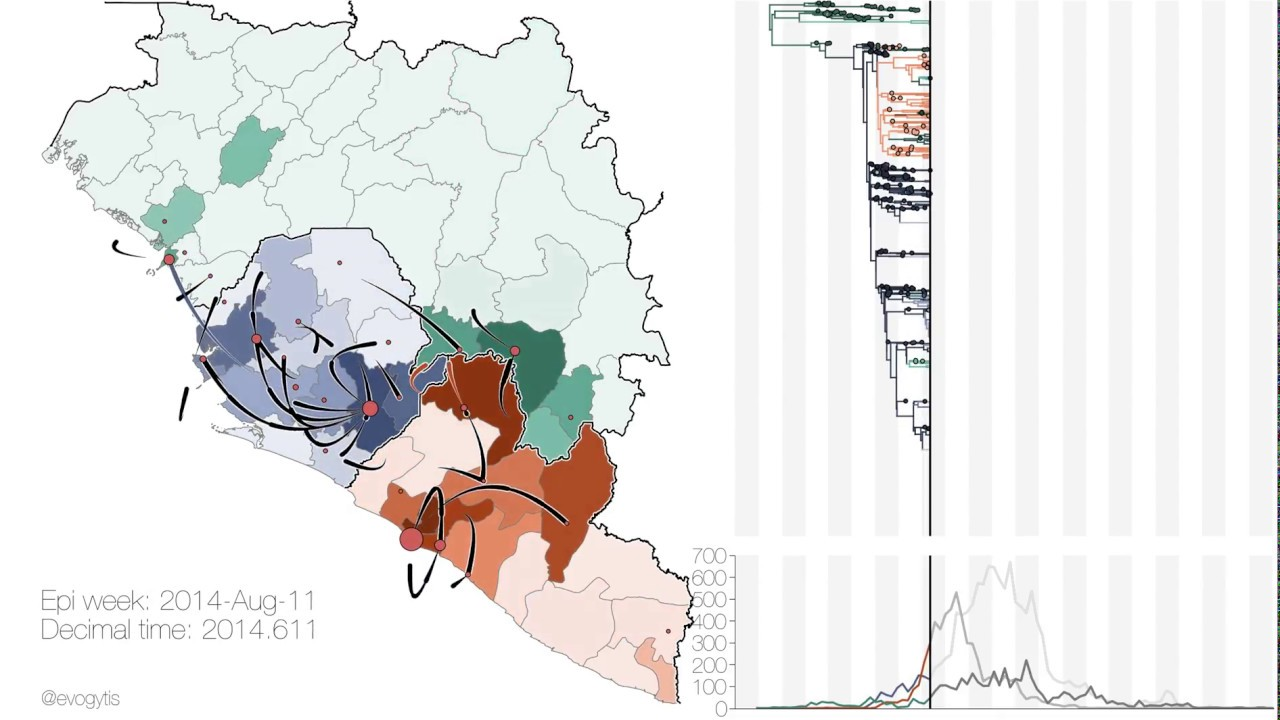
\includegraphics{./Figs/matplot1.png}
\end{frame}

\begin{frame}{Visualizimi i të Dhënave me Matplotlib}
\protect\hypertarget{visualizimi-i-tuxeb-dhuxebnave-me-matplotlib-2}{}
\begin{itemize}
\item
  Sasia e informacionit në këtë vizualizim kompleks është thjesht e
  mahnitshme!
\item
  Ky vizualizim u krijua duke përdorur \textbf{Matplotlib}, një
  bibliotekë Python që përdoret gjerësisht për të vizualizuar të dhënat.
\end{itemize}
\end{frame}

\begin{frame}{Visualizimi i të Dhënave me Matplotlib}
\protect\hypertarget{visualizimi-i-tuxeb-dhuxebnave-me-matplotlib-3}{}
\begin{itemize}
\item
  Ka shumë biblioteka softuerike që vizualizojnë të dhëna.
\item
  Një nga avantazhet kryesore të Matplotlib është që ju jep kontroll të
  plotë mbi atributet e grafikut tuaj.
\item
  Kjo ju lejon të personalizoni dhe kontrolloni çdo veçori të
  vizualizimeve tuaja.
\end{itemize}
\end{frame}

\begin{frame}{Prezantimi i ndërfaqes pyplot}
\protect\hypertarget{prezantimi-i-nduxebrfaqes-pyplot}{}
\begin{itemize}
\item
  Ka shumë mënyra të ndryshme për të përdorur Matplotlib.
\item
  Në këtë leksion, ne do të përdorim ndërfaqen kryesore të orientuar
  ndaj objekteve.
\item
  Kjo ndërfaqe ofrohet përmes nën-modulit \textbf{pyplot}.
\end{itemize}
\end{frame}

\begin{frame}[fragile]{Prezantimi i ndërfaqes pyplot}
\protect\hypertarget{prezantimi-i-nduxebrfaqes-pyplot-1}{}
\begin{verbatim}
import matplotlib.pyplot as plt
\end{verbatim}
\end{frame}

\begin{frame}{Prezantimi i ndërfaqes pyplot}
\protect\hypertarget{prezantimi-i-nduxebrfaqes-pyplot-2}{}
\begin{itemize}
\item
  Këtu, ne importojmë këtë nën-modul dhe e quajmë \textbf{plt}.
\item
  Edhe pse përdorimi i emrit \textbf{plt} nuk është i domosdoshëm për të
  funksionuar, kjo praktikë këshillohet.
\end{itemize}
\end{frame}

\begin{frame}[fragile]{Prezantimi i ndërfaqes pyplot}
\protect\hypertarget{prezantimi-i-nduxebrfaqes-pyplot-3}{}
\AddToHookNext{env/Highlighting/begin}{\scriptsize}

\begin{Shaded}
\begin{Highlighting}[]
\ImportTok{import}\NormalTok{ matplotlib.pyplot }\ImportTok{as}\NormalTok{ plt}
\NormalTok{fig, ax }\OperatorTok{=}\NormalTok{ plt.subplots()}
\NormalTok{plt.show()}
\end{Highlighting}
\end{Shaded}

\begin{itemize}
\item
  Komanda \textbf{plt.subplots()}, kur thirret pa asnjë input, krijon dy
  objekte të ndryshme:

  \begin{itemize}
  \tightlist
  \item
    një objekt \textbf{Figure} dhe një objekt \textbf{Axes}.
  \end{itemize}
\end{itemize}
\end{frame}

\begin{frame}{Prezantimi i ndërfaqes pyplot}
\protect\hypertarget{prezantimi-i-nduxebrfaqes-pyplot-4}{}
\begin{itemize}
\item
  Objekti \textbf{Figure} është një konteiner që mban gjithçka që shihni
  në faqe.
\item
  Ndërkohë, \textbf{Axes} është pjesa e faqes që mban të dhënat.
\item
  Është kanavaca në të cilën do të vizatoni me të dhënat tuaja, për t'i
  vizualizuar ato.
\end{itemize}
\end{frame}

\begin{frame}{Prezantimi i ndërfaqes pyplot}
\protect\hypertarget{prezantimi-i-nduxebrfaqes-pyplot-5}{}
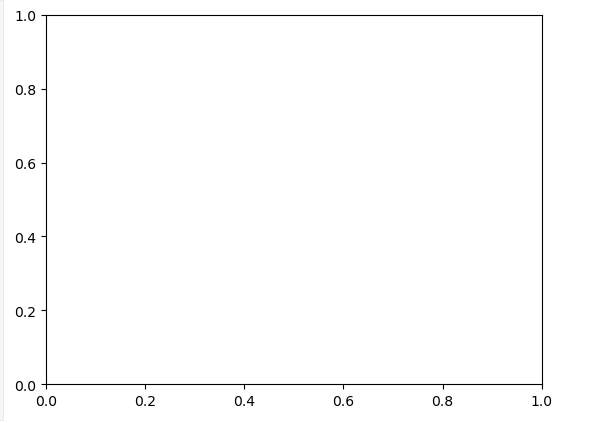
\includegraphics{./Figs/matplot2.png}

\begin{itemize}
\item
  Këtu, mund të shihni një Figurë me Axes të zbrazët.
\item
  Ende nuk është shtuar asnjë të dhënë.
\end{itemize}
\end{frame}

\begin{frame}[fragile]{Shtimi i të dhënave në axes}
\protect\hypertarget{shtimi-i-tuxeb-dhuxebnave-nuxeb-axes}{}
\begin{itemize}
\tightlist
\item
  Le të shtojmë disa të dhëna në figurën tonë.
\end{itemize}

\AddToHookNext{env/Highlighting/begin}{\scriptsize}

\begin{Shaded}
\begin{Highlighting}[]
\CommentTok{\# edited/added}
\ImportTok{import}\NormalTok{ pandas }\ImportTok{as}\NormalTok{ pd}
\ImportTok{import}\NormalTok{ calendar}
\NormalTok{seattle\_weather }\OperatorTok{=}\NormalTok{ pd.read\_csv(}\StringTok{"data/visualisation/seattle\_weather.csv"}\NormalTok{)}
\NormalTok{seattle\_weather }\OperatorTok{=}\NormalTok{ seattle\_weather[seattle\_weather[}\StringTok{\textquotesingle{}STATION\textquotesingle{}}\NormalTok{] }\OperatorTok{==} \StringTok{\textquotesingle{}USW00094290\textquotesingle{}}\NormalTok{]}
\NormalTok{seattle\_weather[}\StringTok{\textquotesingle{}MONTH\textquotesingle{}}\NormalTok{] }\OperatorTok{=}\NormalTok{ seattle\_weather[}\StringTok{\textquotesingle{}DATE\textquotesingle{}}\NormalTok{]}
\end{Highlighting}
\end{Shaded}
\end{frame}

\begin{frame}{Shtimi i të dhënave në axes}
\protect\hypertarget{shtimi-i-tuxeb-dhuxebnave-nuxeb-axes-1}{}
\begin{itemize}
\item
  Këtu ka disa të dhëna.
\item
  Ky është një DataFrame që përmban informacion mbi motin në qytetin e
  Seattle në muajt e ndryshëm të vitit.
\item
  Kolona ``MONTH'' përmban emrat e tre shkronjave të muajve të vitit.
\item
  Kolona ````MLY-TAVG-NORMAL'' përmban temperaturat në këta muaj, në
  gradë Fahrenheit, të matur në një periudhë dhjetëvjeçare.
\end{itemize}
\end{frame}

\begin{frame}{Shtimi i të dhënave në axes}
\protect\hypertarget{shtimi-i-tuxeb-dhuxebnave-nuxeb-axes-2}{}
\begin{itemize}
\item
  Për të shtuar të dhënat në Axes, ne thërrasim një komandë grafiku.
\item
  Komandat e grafikut janë metodat e objektit Axes.
\end{itemize}
\end{frame}

\begin{frame}[fragile]{Shtimi i të dhënave në axes}
\protect\hypertarget{shtimi-i-tuxeb-dhuxebnave-nuxeb-axes-3}{}
\AddToHookNext{env/Highlighting/begin}{\scriptsize}

\begin{Shaded}
\begin{Highlighting}[]
\ImportTok{import}\NormalTok{ matplotlib.pyplot }\ImportTok{as}\NormalTok{ plt}

\NormalTok{fig, ax }\OperatorTok{=}\NormalTok{ plt.subplots()}

\NormalTok{ax.plot(seattle\_weather[}\StringTok{"MONTH"}\NormalTok{], seattle\_weather[}\StringTok{"MLY{-}PRCP{-}NORMAL"}\NormalTok{])}
\end{Highlighting}
\end{Shaded}
\end{frame}

\begin{frame}{Shtimi i të dhënave në axes}
\protect\hypertarget{shtimi-i-tuxeb-dhuxebnave-nuxeb-axes-4}{}
\begin{itemize}
\item
  Për shembull, këtu ne thërrasim metodën e quajtur \textbf{plot} me
  kolonën e muajit si argumentin e parë dhe kolonën e temperaturës si
  argumentin e dytë.
\item
  Thërrasim funksionin \textbf{plt.show()} për të treguar efektin e
  komandës së vizatimit.
\item
  Kjo shton një vijë në grafik.
\end{itemize}
\end{frame}

\begin{frame}{Shtimi i të dhënave në axes}
\protect\hypertarget{shtimi-i-tuxeb-dhuxebnave-nuxeb-axes-5}{}
\begin{itemize}
\item
  Dimensioni horizontal i grafikut paraqet muajt sipas radhës së tyre
  dhe lartësia e vijës në çdo muaj përfaqëson temperaturën mesatare.
\item
  Tendencat në të dhënat tani janë shumë më të qarta seç ishin vetëm
  duke lexuar temperaturat nga tabela.
\end{itemize}
\end{frame}

\begin{frame}{Shtimi i më shumë të dhënave}
\protect\hypertarget{shtimi-i-muxeb-shumuxeb-tuxeb-dhuxebnave}{}
\begin{itemize}
\item
  Nëse dëshironi, mund të shtoni më shumë të dhëna në grafik.
\item
  Për shembull, ne gjithashtu kemi një tabelë që ruajt të dhëna rreth
  temperaturave mesatare në qytetin e Austin, Teksas.
\item
  Ne shtojmë këto të dhëna në axes duke thirrur përsëri metodën
  \textbf{plot}.
\end{itemize}
\end{frame}

\begin{frame}[fragile]{Shtimi i më shumë të dhënave}
\protect\hypertarget{shtimi-i-muxeb-shumuxeb-tuxeb-dhuxebnave-1}{}
\AddToHookNext{env/Highlighting/begin}{\scriptsize}

\begin{Shaded}
\begin{Highlighting}[]
\NormalTok{austin\_weather }\OperatorTok{=}\NormalTok{ pd.read\_csv(}\StringTok{"data/visualisation/austin\_weather.csv"}\NormalTok{)}
\NormalTok{austin\_weather[}\StringTok{\textquotesingle{}MONTH\textquotesingle{}}\NormalTok{] }\OperatorTok{=}\NormalTok{ austin\_weather[}\StringTok{\textquotesingle{}DATE\textquotesingle{}}\NormalTok{]}
\NormalTok{fig, ax }\OperatorTok{=}\NormalTok{ plt.subplots()}
\NormalTok{ax.plot(seattle\_weather1[}\StringTok{"MONTH"}\NormalTok{], seattle\_weather1[}\StringTok{"MLY{-}TAVG{-}NORMAL"}\NormalTok{])}
\NormalTok{ax.plot(austin\_weather[}\StringTok{"MONTH"}\NormalTok{], austin\_weather[}\StringTok{"MLY{-}PRCP{-}NORMAL"}\NormalTok{])}
\NormalTok{plt.show()}
\end{Highlighting}
\end{Shaded}
\end{frame}

\begin{frame}{Vendosja e të gjitha bashkë}
\protect\hypertarget{vendosja-e-tuxeb-gjitha-bashkuxeb}{}
Ja se si do të duket i gjithë kodi për të krijuar këtë figurë.

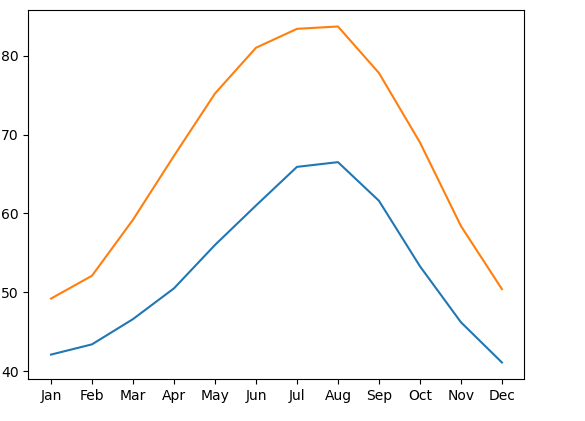
\includegraphics{./Figs/matplot3.png}
\end{frame}

\begin{frame}{Ushtrim : Përdorimi i matplotlib.pyplot}
\protect\hypertarget{ushtrim-puxebrdorimi-i-matplotlib.pyplot}{}
\begin{itemize}
\item
  Në këtë ushtrim, do të përqendrohemi te përdorimi i
  \textbf{matplotlib.pyplot} për të krijuar objekte \textbf{Figure} dhe
  \textbf{Axes}.
\item
  \textbf{Matplotlib.pyplot} ofron fleksibilitet në krijimin dhe
  personalizimin e vizualizimeve të të dhënave.
\end{itemize}
\end{frame}

\begin{frame}[fragile]{Instruksionet}
\protect\hypertarget{instruksionet}{}
\begin{enumerate}
\item
  Importoni API-n matplotlib.pyplot, duke përdorur emrin konvencional
  \texttt{plt}.
\item
  Krijoni objekte Figure dhe Axes duke përdorur funksionin
  \texttt{plt.subplots}.
\item
  Shfaqni rezultatin, një set bosh të akseve, duke përdorur funksionin
  \texttt{plt.show}.
\end{enumerate}
\end{frame}

\begin{frame}[fragile]{Zgjidhje}
\protect\hypertarget{zgjidhje}{}
\AddToHookNext{env/Highlighting/begin}{\scriptsize}

\begin{Shaded}
\begin{Highlighting}[]
\ImportTok{import}\NormalTok{ matplotlib.pyplot }\ImportTok{as}\NormalTok{ plt  }\CommentTok{\# Importo matplotlib.pyplot si plt}
\NormalTok{fig, ax }\OperatorTok{=}\NormalTok{ plt.subplots()  }\CommentTok{\# Krijo një figurë dhe akset}
\NormalTok{plt.show()  }\CommentTok{\# Shfaq një set bosh të akseve}
\end{Highlighting}
\end{Shaded}
\end{frame}

\begin{frame}[fragile]{Ushtrimi: Shtimi i të Dhënave në Objektin Axes}
\protect\hypertarget{ushtrimi-shtimi-i-tuxeb-dhuxebnave-nuxeb-objektin-axes}{}
\begin{itemize}
\item
  Në këtë ushtrim, do të mësojmë se si të shtojmë të dhëna në një objekt
  Axes duke përdorur metodën \texttt{plot}.
\item
  Do të përdorim të dhënat nga dy qytete amerikane: Seattle dhe Austin
  për të krahasuar reshjet mujore.
\end{itemize}
\end{frame}

\begin{frame}[fragile]{Instruksionet}
\protect\hypertarget{instruksionet-1}{}
\begin{enumerate}
\item
  Importoni nën-modulin matplotlib.pyplot si \texttt{plt}.
\item
  Krijoni një figurë dhe një objekt Axes duke thirrur
  \texttt{plt.subplots}.
\item
  Shtoni të dhënat nga DataFrame \texttt{seattle\_weather} duke përdorur
  metodën \texttt{plot} të objektit Axes.
\item
  Shtoni të dhënat nga DataFrame \texttt{austin\_weather} në mënyrë të
  ngjashme dhe përdorni \texttt{plt.show} për të shfaqur rezultatin.
\end{enumerate}
\end{frame}

\begin{frame}[fragile]{Zgjidhje}
\protect\hypertarget{zgjidhje-1}{}
\AddToHookNext{env/Highlighting/begin}{\scriptsize}

\begin{Shaded}
\begin{Highlighting}[]
\ImportTok{import}\NormalTok{ matplotlib.pyplot }\ImportTok{as}\NormalTok{ plt  }\CommentTok{\# Importo matplotlib.pyplot si plt}

\CommentTok{\# Krijoni një figurë dhe një objekt Axes}
\NormalTok{fig, ax }\OperatorTok{=}\NormalTok{ plt.subplots()}

\CommentTok{\# Shtoni të dhënat e reshjeve për Seattle}
\NormalTok{ax.plot(seattle\_weather[}\StringTok{"MONTH"}\NormalTok{], seattle\_weather[}\StringTok{"MLY{-}PRCP{-}NORMAL"}\NormalTok{], label}\OperatorTok{=}\StringTok{"Seattle"}\NormalTok{)}

\CommentTok{\# Shtoni të dhënat e reshjeve për Austin}
\NormalTok{ax.plot(austin\_weather[}\StringTok{"MONTH"}\NormalTok{], austin\_weather[}\StringTok{"MLY{-}PRCP{-}NORMAL"}\NormalTok{], label}\OperatorTok{=}\StringTok{"Austin"}\NormalTok{)}

\CommentTok{\# Shtoni një legjendë për të shpjeguar etiketat}
\NormalTok{ax.legend()}

\CommentTok{\# Shfaqni figurën për të parë rezultatin}
\NormalTok{plt.show()}
\end{Highlighting}
\end{Shaded}
\end{frame}

\hypertarget{personalizimi-i-grafikuxebve}{%
\section{Personalizimi i Grafikëve}\label{personalizimi-i-grafikuxebve}}

\begin{frame}{Personalizimi i Grafikëve}
\protect\hypertarget{personalizimi-i-grafikuxebve-1}{}
Tani që dini se si të shtoni të dhëna në një grafik, le të fillojmë të
personalizojmë grafikët tuaj.
\end{frame}

\begin{frame}{Personalizimi i Pamjes së të Dhënave}
\protect\hypertarget{personalizimi-i-pamjes-suxeb-tuxeb-dhuxebnave}{}
\begin{itemize}
\item
  Së pari, le të personalizojmë pamjen e të dhënave në grafik.
\item
  Një problem që mund të përmirësohet është se të dhënat duken të
  vazhdueshme, por në të vërtetë janë matur vetëm në intervale mujore.
\end{itemize}
\end{frame}

\begin{frame}{Personalizimi i Pamjes së të Dhënave}
\protect\hypertarget{personalizimi-i-pamjes-suxeb-tuxeb-dhuxebnave-1}{}
\begin{itemize}
\tightlist
\item
  Një mënyrë për të treguar këtë është duke shtuar shënjues që tregojnë
  se ku janë të dhënat dhe cilat pjesë janë thjesht linja që lidhin
  pikat e të dhënave.
\end{itemize}
\end{frame}

\begin{frame}[fragile]{Shtimi i Shënjuesve}
\protect\hypertarget{shtimi-i-shuxebnjuesve}{}
\begin{itemize}
\item
  Metoda \texttt{plot} ka një argument opsional \texttt{marker}, që ju
  lejon të shtoni shënjues në grafik dhe gjithashtu të zgjidhni llojin e
  shënjuesve.
\item
  Për shembull, duke përdorur shkronjën e vogël ``o'', mund të përdorni
  rrethin si shënjues.
\end{itemize}
\end{frame}

\begin{frame}[fragile]{Shtimi i Shënjuesve}
\protect\hypertarget{shtimi-i-shuxebnjuesve-1}{}
\AddToHookNext{env/Highlighting/begin}{\scriptsize}

\begin{Shaded}
\begin{Highlighting}[]
\NormalTok{fig, ax }\OperatorTok{=}\NormalTok{ plt.subplots()}

\NormalTok{ax.plot(seattle\_weather[}\StringTok{"MONTH"}\NormalTok{], seattle\_weather[}\StringTok{"MLY{-}TAVG{-}NORMAL"}\NormalTok{],}
\NormalTok{marker}\OperatorTok{=}\StringTok{"o"}\NormalTok{)}

\NormalTok{plt.show()}
\end{Highlighting}
\end{Shaded}
\end{frame}

\begin{frame}[fragile]{Zgjedhja e Shënjuesve}
\protect\hypertarget{zgjedhja-e-shuxebnjuesve}{}
\begin{itemize}
\tightlist
\item
  Nëse përdorni shkronjën e vogël ``v'', do të merrni shënjues në formë
  trekëndëshi që tregojnë poshtë.
\end{itemize}

\AddToHookNext{env/Highlighting/begin}{\scriptsize}

\begin{Shaded}
\begin{Highlighting}[]
\NormalTok{fig, ax }\OperatorTok{=}\NormalTok{ plt.subplots()}

\NormalTok{ax.plot(seattle\_weather[}\StringTok{"MONTH"}\NormalTok{], seattle\_weather[}\StringTok{"MLY{-}TAVG{-}NORMAL"}\NormalTok{],}
\NormalTok{marker}\OperatorTok{=}\StringTok{"v"}\NormalTok{)}

\NormalTok{plt.show()}
\end{Highlighting}
\end{Shaded}

\begin{itemize}
\tightlist
\item
  Për të parë të gjitha stilet e mundshme të shënjuesve, mund të
  vizitoni faqen e dokumentacionit të matplotlib.
\end{itemize}
\end{frame}

\begin{frame}[fragile]{Vendosja e Stilit të Vijës}
\protect\hypertarget{vendosja-e-stilit-tuxeb-vijuxebs}{}
\begin{itemize}
\item
  Për të ndryshuar pamjen e linjave që lidhin shënjuesit, mund të
  përdorni argumentin \texttt{linestyle}.
\item
  Për shembull, dy viza do të thotë se linja duhet të jetë me viza.
\item
  Për stile të tjera të linjës, mund të shikoni dokumentacionin e
  matplotlib.
\end{itemize}
\end{frame}

\begin{frame}[fragile]{Vendosja e Stilit të Vijës}
\protect\hypertarget{vendosja-e-stilit-tuxeb-vijuxebs-1}{}
\AddToHookNext{env/Highlighting/begin}{\scriptsize}

\begin{Shaded}
\begin{Highlighting}[]
\NormalTok{fig, ax }\OperatorTok{=}\NormalTok{ plt.subplots()}

\NormalTok{ax.plot(austin\_weather[}\StringTok{"MONTH"}\NormalTok{], austin\_weather[}\StringTok{"MLY{-}TAVG{-}NORMAL"}\NormalTok{],}
\NormalTok{marker}\OperatorTok{=}\StringTok{"v"}\NormalTok{, linestyle}\OperatorTok{=}\StringTok{"{-}{-}"}\NormalTok{)}

\NormalTok{plt.show()}
\end{Highlighting}
\end{Shaded}
\end{frame}

\begin{frame}[fragile]{Eliminimi i Linjave me \texttt{linestyle}}
\protect\hypertarget{eliminimi-i-linjave-me-linestyle}{}
Nëse dëshironi të hiqni linjat, mund të përdorni fjalën ``None'' në
argumentin \texttt{linestyle}.

\AddToHookNext{env/Highlighting/begin}{\scriptsize}

\begin{Shaded}
\begin{Highlighting}[]
\NormalTok{fig, ax }\OperatorTok{=}\NormalTok{ plt.subplots()}

\NormalTok{ax.plot(austin\_weather[}\StringTok{"MONTH"}\NormalTok{], austin\_weather[}\StringTok{"MLY{-}TAVG{-}NORMAL"}\NormalTok{],}
\NormalTok{marker}\OperatorTok{=}\StringTok{"v"}\NormalTok{, linestyle}\OperatorTok{=}\StringTok{"None"}\NormalTok{)}

\NormalTok{plt.show()}
\end{Highlighting}
\end{Shaded}
\end{frame}

\begin{frame}{Zgjedhja e Ngjyrës}
\protect\hypertarget{zgjedhja-e-ngjyruxebs}{}
\begin{itemize}
\item
  Ju gjithashtu mund të zgjidhni ngjyrën që dëshironi për të dhënat.
\item
  Për shembull, për të treguar të dhënat në të kuqe, mund të përdorni
  shkronjën ``r''.
\end{itemize}
\end{frame}

\begin{frame}[fragile]{Zgjedhja e Ngjyrës}
\protect\hypertarget{zgjedhja-e-ngjyruxebs-1}{}
\AddToHookNext{env/Highlighting/begin}{\scriptsize}

\begin{Shaded}
\begin{Highlighting}[]
\NormalTok{fig, ax }\OperatorTok{=}\NormalTok{ plt.subplots()}

\NormalTok{ax.plot(seattle\_weather[}\StringTok{"MONTH"}\NormalTok{], seattle\_weather[}\StringTok{"MLY{-}TAVG{-}NORMAL"}\NormalTok{],}
\NormalTok{marker}\OperatorTok{=}\StringTok{"o"}\NormalTok{, linestyle}\OperatorTok{=}\StringTok{"None"}\NormalTok{, color}\OperatorTok{=}\StringTok{"r"}\NormalTok{)}

\NormalTok{plt.show()}
\end{Highlighting}
\end{Shaded}
\end{frame}

\begin{frame}[fragile]{Personalizimi i Etiketave të Akseve}
\protect\hypertarget{personalizimi-i-etiketave-tuxeb-akseve}{}
\begin{itemize}
\item
  Është e rëndësishme të etiketoni akseset.
\item
  Për këtë, mund të përdorni metodën \texttt{set\_xlabel} për të
  vendosur etiketën e aksit x dhe \texttt{set\_ylabel} për aksin y.
\end{itemize}
\end{frame}

\begin{frame}[fragile]{Vendosja e Etiketës së Aksit Y}
\protect\hypertarget{vendosja-e-etiketuxebs-suxeb-aksit-y}{}
Për të vendosur etiketën e aksit y, përdorni \texttt{set\_ylabel} dhe
vendosni tekstin që përshtatet me vlerat e të dhënave.
\end{frame}

\begin{frame}[fragile]{Personalizimi i Etiketave të Akseve}
\protect\hypertarget{personalizimi-i-etiketave-tuxeb-akseve-1}{}
\AddToHookNext{env/Highlighting/begin}{\scriptsize}

\begin{Shaded}
\begin{Highlighting}[]
\NormalTok{fig, ax }\OperatorTok{=}\NormalTok{ plt.subplots()}

\NormalTok{ax.plot(seattle\_weather[}\StringTok{"MONTH"}\NormalTok{], seattle\_weather[}\StringTok{"MLY{-}TAVG{-}NORMAL"}\NormalTok{],}
\NormalTok{marker}\OperatorTok{=}\StringTok{"o"}\NormalTok{, linestyle}\OperatorTok{=}\StringTok{"None"}\NormalTok{, color}\OperatorTok{=}\StringTok{"r"}\NormalTok{)}
\NormalTok{ax.set\_xlabel(}\StringTok{"Koha (Muaj)"}\NormalTok{)}
\NormalTok{ax.set\_ylabel(}\StringTok{"Temperatura mesatare (Grade F)"}\NormalTok{)}

\NormalTok{plt.show()}
\end{Highlighting}
\end{Shaded}
\end{frame}

\begin{frame}[fragile]{Shtimi i Një Titulli}
\protect\hypertarget{shtimi-i-njuxeb-titulli}{}
Për të shtuar një titull në aksin tuaj, mund të përdorni
\texttt{set\_title} për të dhënë informacion shtesë dhe kontekst për
vizualizimin tuaj.

\AddToHookNext{env/Highlighting/begin}{\scriptsize}

\begin{Shaded}
\begin{Highlighting}[]
\NormalTok{fig, ax }\OperatorTok{=}\NormalTok{ plt.subplots()}

\NormalTok{ax.plot(seattle\_weather[}\StringTok{"MONTH"}\NormalTok{], seattle\_weather[}\StringTok{"MLY{-}TAVG{-}NORMAL"}\NormalTok{],}
\NormalTok{marker}\OperatorTok{=}\StringTok{"o"}\NormalTok{, linestyle}\OperatorTok{=}\StringTok{"None"}\NormalTok{, color}\OperatorTok{=}\StringTok{"r"}\NormalTok{)}
\NormalTok{ax.set\_xlabel(}\StringTok{"Koha (Muaj)"}\NormalTok{)}
\NormalTok{ax.set\_ylabel(}\StringTok{"Temperatura mesatare (Grade F)"}\NormalTok{)}
\NormalTok{ax.set\_title(}\StringTok{"Moti ne Seattle"}\NormalTok{)}
\NormalTok{plt.show()}
\end{Highlighting}
\end{Shaded}
\end{frame}

\begin{frame}{Praktikoni Personalizimin e Grafikëve!}
\protect\hypertarget{praktikoni-personalizimin-e-grafikuxebve}{}
Tani që keni parë disa shembuj të personalizimit të pamjes së të dhënave
dhe etiketat e aksëve, është koha për të praktikuar këto koncepte.
\end{frame}

\begin{frame}{Ushtrimi: Personalizimi i Pamjes së të Dhënave}
\protect\hypertarget{ushtrimi-personalizimi-i-pamjes-suxeb-tuxeb-dhuxebnave}{}
Në këtë ushtrim, do të personalizojmë pamjen e shënjuesve, stilin e
linjës, dhe ngjyrën e linjave dhe shënjuesve për të dhënat.
\end{frame}

\begin{frame}[fragile]{Instruksionet}
\protect\hypertarget{instruksionet-2}{}
\begin{enumerate}
\item
  Përdorni \texttt{ax.plot} për të grafikuar ``MLY-PRCP-NORMAL'' kundër
  ``MONTHS'' për të dy DataFrame-t: \texttt{seattle\_weather} dhe
  \texttt{austin\_weather}.
\item
  Përdorni argumentin \texttt{color} për të vendosur ngjyrën e të
  dhënave të Seattle në blu (`b') dhe të Austin në të kuqe (`r').
\item
  Përdorni argumentin \texttt{marker} për të vendosur shënjuesit e
  Seattle në formë rrethi (`o') dhe të Austin në formë trekëndëshi që
  tregon poshtë (`v').
\item
  Përdorni argumentin \texttt{linestyle} për të përdorur linjat me viza
  (`--') për të dhënat nga të dy qytetet.
\end{enumerate}
\end{frame}

\begin{frame}[fragile]{Zgjidhje}
\protect\hypertarget{zgjidhje-2}{}
\AddToHookNext{env/Highlighting/begin}{\scriptsize}

\begin{Shaded}
\begin{Highlighting}[]
\NormalTok{fig, ax }\OperatorTok{=}\NormalTok{ plt.subplots()}
\NormalTok{ax.plot(seattle\_weather[}\StringTok{"MONTH"}\NormalTok{], seattle\_weather[}\StringTok{"MLY{-}PRCP{-}NORMAL"}\NormalTok{],}
\NormalTok{        color}\OperatorTok{=}\StringTok{\textquotesingle{}b\textquotesingle{}}\NormalTok{, marker}\OperatorTok{=}\StringTok{\textquotesingle{}o\textquotesingle{}}\NormalTok{, linestyle}\OperatorTok{=}\StringTok{\textquotesingle{}{-}{-}\textquotesingle{}}\NormalTok{)}

\NormalTok{ax.plot(austin\_weather[}\StringTok{"MONTH"}\NormalTok{], austin\_weather[}\StringTok{"MLY{-}PRCP{-}NORMAL"}\NormalTok{],}
\NormalTok{        color}\OperatorTok{=}\StringTok{\textquotesingle{}r\textquotesingle{}}\NormalTok{, marker}\OperatorTok{=}\StringTok{\textquotesingle{}v\textquotesingle{}}\NormalTok{, linestyle}\OperatorTok{=}\StringTok{\textquotesingle{}{-}{-}\textquotesingle{}}\NormalTok{)}

\NormalTok{plt.show()}
\end{Highlighting}
\end{Shaded}
\end{frame}

\begin{frame}[fragile]{Ushtrimi: Personalizimi i Etiketave të Aksëve dhe
Shtimi i Titullit}
\protect\hypertarget{ushtrimi-personalizimi-i-etiketave-tuxeb-aksuxebve-dhe-shtimi-i-titullit}{}
\begin{itemize}
\item
  Në këtë ushtrim, do të personalizojmë etiketat e aksëve duke përdorur
  metodat \texttt{set\_xlabel} dhe \texttt{set\_ylabel}.
\item
  Gjithashtu, do të shtojmë një titull duke përdorur metodën
  \texttt{set\_title}.
\end{itemize}
\end{frame}

\begin{frame}[fragile]{Instruksionet}
\protect\hypertarget{instruksionet-3}{}
\begin{enumerate}
\item
  Përdorni metodën \texttt{set\_xlabel} për të shtuar etiketën ``Koha
  (muaj)''.
\item
  Përdorni metodën \texttt{set\_ylabel} për të shtuar etiketën ``Reshje
  (inç)''.
\item
  Përdorni metodën \texttt{set\_title} për të shtuar titullin ``Moti në
  Austin dhe Seattle''.
\end{enumerate}
\end{frame}

\begin{frame}[fragile]{Zgjidhje}
\protect\hypertarget{zgjidhje-3}{}
\AddToHookNext{env/Highlighting/begin}{\scriptsize}

\begin{Shaded}
\begin{Highlighting}[]
\NormalTok{fig, ax }\OperatorTok{=}\NormalTok{ plt.subplots()}
\NormalTok{ax.plot(seattle\_weather[}\StringTok{"MONTH"}\NormalTok{], seattle\_weather[}\StringTok{"MLY{-}PRCP{-}NORMAL"}\NormalTok{])}
\NormalTok{ax.plot(austin\_weather[}\StringTok{"MONTH"}\NormalTok{], austin\_weather[}\StringTok{"MLY{-}PRCP{-}NORMAL"}\NormalTok{])}

\NormalTok{ax.set\_xlabel(}\StringTok{"Koha (Muaj)"}\NormalTok{)}

\NormalTok{ax.set\_ylabel(}\StringTok{"Rreshjet (inch)"}\NormalTok{)}

\NormalTok{ax.set\_title(}\StringTok{"Moti ne Austin dhe Seattle"}\NormalTok{)}

\NormalTok{plt.show()}
\end{Highlighting}
\end{Shaded}
\end{frame}

\hypertarget{nuxebngrafikuxebt-pjesuxebt-e-vogla}{%
\section{Nëngrafikët: Pjesët e
vogla}\label{nuxebngrafikuxebt-pjesuxebt-e-vogla}}

\begin{frame}{Pjesët e vogla (Small Multiples)}
\protect\hypertarget{pjesuxebt-e-vogla-small-multiples}{}
Ndonjëherë, shtimi i më shumë të dhënave në një grafik mund ta bëjë atë
shumë të ngarkuar, duke fshehur modelet në vend që t'i shfaqë ato.
\end{frame}

\begin{frame}[fragile]{Shtimi i të Dhënave}
\protect\hypertarget{shtimi-i-tuxeb-dhuxebnave}{}
\begin{itemize}
\tightlist
\item
  Për shembull, le të eksplorojmë të dhënat që kemi për motin në
  Seattle.
\end{itemize}

\AddToHookNext{env/Highlighting/begin}{\scriptsize}

\begin{Shaded}
\begin{Highlighting}[]
\NormalTok{fig, ax }\OperatorTok{=}\NormalTok{ plt.subplots()}
\NormalTok{ax.plot(seattle\_weather[}\StringTok{"MONTH"}\NormalTok{], seattle\_weather[}\StringTok{"MLY{-}PRCP{-}NORMAL"}\NormalTok{], color}\OperatorTok{=}\StringTok{\textquotesingle{}b\textquotesingle{}}\NormalTok{)}
\NormalTok{ax.set\_xlabel(}\StringTok{"Time (months)"}\NormalTok{)}
\NormalTok{ax.set\_ylabel(}\StringTok{"Precipitation (inches)"}\NormalTok{)}
\NormalTok{plt.show()}
\end{Highlighting}
\end{Shaded}

\begin{itemize}
\tightlist
\item
  Këtu, ne krijuam grafik për reshjet mesatare gjatë vitit.
\end{itemize}
\end{frame}

\begin{frame}[fragile]{Shtimi i të Dhënave}
\protect\hypertarget{shtimi-i-tuxeb-dhuxebnave-1}{}
\begin{itemize}
\item
  Por nëse dëshirojmë të shtojmë të dhëna shtesë, si psh diapazoni i
  vlerave?
\item
  Në këtë rast, mund të shtojmë percentilin e 25-të dhe të 75-të me vija
  të ndërprera mbi dhe poshtë mesatares.
\item
  Çfarë do të ndodhte nëse do të krahasoheshin me Austin?
\end{itemize}

\AddToHookNext{env/Highlighting/begin}{\scriptsize}

\begin{Shaded}
\begin{Highlighting}[]
\NormalTok{fig, ax }\OperatorTok{=}\NormalTok{ plt.subplots()}
\NormalTok{ax.plot(austin\_weather[}\StringTok{"MONTH"}\NormalTok{], austin\_weather[}\StringTok{"MLY{-}PRCP{-}NORMAL"}\NormalTok{],        color}\OperatorTok{=}\StringTok{\textquotesingle{}r\textquotesingle{}}\NormalTok{)}
\NormalTok{ax.plot(austin\_weather[}\StringTok{"MONTH"}\NormalTok{], austin\_weather[}\StringTok{"MLY{-}PRCP{-}25PCTL"}\NormalTok{],         linestyle}\OperatorTok{=}\StringTok{\textquotesingle{}{-}{-}\textquotesingle{}}\NormalTok{, color}\OperatorTok{=}\StringTok{\textquotesingle{}r\textquotesingle{}}\NormalTok{)}
\NormalTok{ax.plot(austin\_weather[}\StringTok{"MONTH"}\NormalTok{], austin\_weather[}\StringTok{"MLY{-}PRCP{-}75PCTL"}\NormalTok{],         linestyle}\OperatorTok{=}\StringTok{\textquotesingle{}{-}{-}\textquotesingle{}}\NormalTok{, color}\OperatorTok{=}\StringTok{\textquotesingle{}r\textquotesingle{}}\NormalTok{)}
\NormalTok{plt.show()}
\end{Highlighting}
\end{Shaded}
\end{frame}

\begin{frame}{Shumë të Dhëna!}
\protect\hypertarget{shumuxeb-tuxeb-dhuxebna}{}
\begin{itemize}
\item
  Është një rrëmujë.
\item
  Ka shumë të dhëna në këtë grafik.
\item
  Një mënyrë për ta kapërcyer këtë është të përdorni plotës të vegjël
  (small multiples), që janë grafikë të vegjël që tregojnë të dhëna të
  ngjashme në kushte të ndryshme.
\end{itemize}
\end{frame}

\begin{frame}[fragile]{Nëngrafikë me \texttt{plt.subplots}}
\protect\hypertarget{nuxebngrafikuxeb-me-plt.subplots}{}
\begin{itemize}
\item
  Në Matplotlib, Nëngrafikët janë quajtur gjithashtu plotës të vegjël.
\item
  Metoda që i krijon ato është \texttt{plt.subplots}.
\item
  Për të krijuar një rrjet subplots me rreshta dhe kolona, mund të
  përdorni argumentet për të përcaktuar formën.
\end{itemize}
\end{frame}

\begin{frame}[fragile]{Nëngrafikë me \texttt{plt.subplots}}
\protect\hypertarget{nuxebngrafikuxeb-me-plt.subplots-1}{}
\AddToHookNext{env/Highlighting/begin}{\scriptsize}

\begin{Shaded}
\begin{Highlighting}[]
\ImportTok{import}\NormalTok{ matplotlib.pyplot }\ImportTok{as}\NormalTok{ plt  }\CommentTok{\# Importo matplotlib.pyplot si plt}
\CommentTok{\# Krijoni një figurë me tre rreshta dhe dy kolona}
\NormalTok{fig, ax }\OperatorTok{=}\NormalTok{ plt.subplots(}\DecValTok{3}\NormalTok{, }\DecValTok{2}\NormalTok{)  }\CommentTok{\# Krijon tre rreshta dhe dy kolona subplots}
\end{Highlighting}
\end{Shaded}
\end{frame}

\begin{frame}{Shtimi i të Dhënave në Subplots}
\protect\hypertarget{shtimi-i-tuxeb-dhuxebnave-nuxeb-subplots}{}
Tani që kemi një sërë subplots, mund të shtojmë të dhënat duke përdorur
indekse për të adresuar secilin Axes.
\end{frame}

\begin{frame}[fragile]{Nëngrafikë me \texttt{plt.subplots}}
\protect\hypertarget{nuxebngrafikuxeb-me-plt.subplots-2}{}
\AddToHookNext{env/Highlighting/begin}{\scriptsize}

\begin{Shaded}
\begin{Highlighting}[]
\CommentTok{\# Shto të dhënat për Seattle në subplotin e parë}
\NormalTok{ax[}\DecValTok{0}\NormalTok{, }\DecValTok{0}\NormalTok{].plot(seattle\_weather[}\StringTok{"MONTH"}\NormalTok{], seattle\_weather[}\StringTok{"MLY{-}PRCP{-}NORMAL"}\NormalTok{])  }
\end{Highlighting}
\end{Shaded}
\end{frame}

\begin{frame}{Nëngrafikë me \texttt{plt.subplots}}
\protect\hypertarget{nuxebngrafikuxeb-me-plt.subplots-3}{}
\begin{itemize}
\item
  Kur kemi vetëm një rresht ose një kolonë, rezultati do të jetë një
  dimension i vetëm, dhe do të përdorim një indeks për të aksesuar
  elementët.
\item
  Për shembull, për të shtuar etiketat në subplotin e parë dhe të dytë,
  mund të përdorni set\_xlabel dhe set\_ylabel.
\end{itemize}
\end{frame}

\begin{frame}[fragile]{Vendos etiketën e aksit x në subplotin e fundit}
\protect\hypertarget{vendos-etiketuxebn-e-aksit-x-nuxeb-subplotin-e-fundit}{}
\AddToHookNext{env/Highlighting/begin}{\scriptsize}

\begin{Shaded}
\begin{Highlighting}[]
\NormalTok{ax[}\DecValTok{2}\NormalTok{][}\DecValTok{1}\NormalTok{].set\_xlabel(}\StringTok{"Koha (muaj)"}\NormalTok{)}
\end{Highlighting}
\end{Shaded}
\end{frame}

\begin{frame}[fragile]{Zgjedhja e Range të Aksit Y}
\protect\hypertarget{zgjedhja-e-range-tuxeb-aksit-y}{}
Për të siguruar që të gjitha subplots të kenë të njëjtin diapazon të
aksit y, përdorni argumentin sharey=True kur krijoni subplots me
plt.subplots.

\AddToHookNext{env/Highlighting/begin}{\scriptsize}

\begin{Shaded}
\begin{Highlighting}[]
\CommentTok{\# Krijoni një figurë me një range të përbashkët për aksin y}
\NormalTok{fig, ax }\OperatorTok{=}\NormalTok{ plt.subplots(}\DecValTok{2}\NormalTok{, }\DecValTok{1}\NormalTok{, sharey}\OperatorTok{=}\VariableTok{True}\NormalTok{)  }
\end{Highlighting}
\end{Shaded}
\end{frame}

\begin{frame}{Praktika me Subplots!}
\protect\hypertarget{praktika-me-subplots}{}
Tani që keni parë se si të krijoni subplots dhe të shtoni të dhëna në
to, praktikoni krijimin e vizualizimeve me këto koncepte.
\end{frame}

\begin{frame}[fragile]{Ushtrimi: Krijimi i `Small Multiples' me
plt.subplots()}
\protect\hypertarget{ushtrimi-krijimi-i-small-multiples-me-plt.subplots}{}
\begin{itemize}
\item
  Në këtë ushtrim, do të përdorim funksionin \texttt{plt.subplots()} për
  të krijuar një sërë subplots me dy rreshta dhe dy kolona.
\item
  Më pas, do të përdorim të dhënat nga \texttt{seattle\_weather} dhe
  \texttt{austin\_weather} për të plotësuar këto subplots.
\end{itemize}
\end{frame}

\begin{frame}{Instruksionet}
\protect\hypertarget{instruksionet-4}{}
\begin{enumerate}
\item
  Krijoni një Figurë dhe një subplots me 2 rreshta dhe 2 kolona.
\item
  Në subplotin e majtë në krye (indeksi 0, 0), shfaqni reshjet mesatare
  për Seattle.
\item
  Në subplotin e djathtë në krye (indeksi 0, 1), shfaqni temperaturat
  mesatare për Seattle.
\item
  Në subplotin e majtë poshtë (indeksi 1, 0), shfaqni reshjet mesatare
  për Austin.
\item
  Në subplotin e djathtë poshtë (indeksi 1, 1), shfaqni temperaturat
  mesatare për Austin.
\end{enumerate}
\end{frame}

\begin{frame}[fragile]{Zgjidhje}
\protect\hypertarget{zgjidhje-4}{}
\AddToHookNext{env/Highlighting/begin}{\scriptsize}

\begin{Shaded}
\begin{Highlighting}[]
\NormalTok{fig, ax }\OperatorTok{=}\NormalTok{ plt.subplots(}\DecValTok{2}\NormalTok{, }\DecValTok{2}\NormalTok{)}


\NormalTok{ax[}\DecValTok{0}\NormalTok{, }\DecValTok{0}\NormalTok{].plot(seattle\_weather[}\StringTok{"MONTH"}\NormalTok{], seattle\_weather[}\StringTok{"MLY{-}PRCP{-}NORMAL"}\NormalTok{])}


\NormalTok{ax[}\DecValTok{0}\NormalTok{, }\DecValTok{1}\NormalTok{].plot(seattle\_weather[}\StringTok{"MONTH"}\NormalTok{], seattle\_weather[}\StringTok{"MLY{-}TAVG{-}NORMAL"}\NormalTok{])}


\NormalTok{ax[}\DecValTok{1}\NormalTok{, }\DecValTok{0}\NormalTok{].plot(austin\_weather[}\StringTok{"MONTH"}\NormalTok{], austin\_weather[}\StringTok{"MLY{-}PRCP{-}NORMAL"}\NormalTok{])}


\NormalTok{ax[}\DecValTok{1}\NormalTok{, }\DecValTok{1}\NormalTok{].plot(austin\_weather[}\StringTok{"MONTH"}\NormalTok{], austin\_weather[}\StringTok{"MLY{-}TAVG{-}NORMAL"}\NormalTok{])}
\NormalTok{plt.show()}
\end{Highlighting}
\end{Shaded}
\end{frame}

\begin{frame}[fragile]{Ushtrimi: `Small Multiples' me Aksin Y të
Përbashkët}
\protect\hypertarget{ushtrimi-small-multiples-me-aksin-y-tuxeb-puxebrbashkuxebt}{}
\begin{itemize}
\item
  Në këtë ushtrim, do të krijojmë një figurë me dy Axes që ndajnë të
  njëjtin aks y.
\item
  Të dhënat janë dhënë në DataFrames \texttt{seattle\_weather} dhe
  \texttt{austin\_weather}.
\end{itemize}
\end{frame}

\begin{frame}{Instruksionet}
\protect\hypertarget{instruksionet-5}{}
\begin{enumerate}
\item
  Krijoni një figurë me dy Axes që ndajnë të njëjtin aks y.
\item
  Shfaqni reshjet mesatare (``MLY-PRCP-NORMAL'') për Seattle me një
  linjë blu të plotë në Axes-in e sipërm.
\item
  Shtoni reshjet e 25-të dhe 75-të percentilit (``MLY-PRCP-25PCTL'' dhe
  ``MLY-PRCP-75PCTL'') në Axes-in e sipërm me linja të ndërprera blu.
\item
  Shfaqni reshjet mesatare për Austin me një linjë të kuqe të plotë në
  Axes-in e poshtëm, dhe shtoni reshjet e 25-të dhe 75-të percentilit me
  linja të ndërprera të kuqe.
\end{enumerate}
\end{frame}

\begin{frame}[fragile]{Zgjidhje}
\protect\hypertarget{zgjidhje-5}{}
\AddToHookNext{env/Highlighting/begin}{\scriptsize}

\begin{Shaded}
\begin{Highlighting}[]
\NormalTok{fig, ax }\OperatorTok{=}\NormalTok{ plt.subplots(}\DecValTok{2}\NormalTok{, }\DecValTok{1}\NormalTok{, sharey}\OperatorTok{=}\VariableTok{True}\NormalTok{)}


\NormalTok{ax[}\DecValTok{0}\NormalTok{].plot(seattle\_weather[}\StringTok{"MONTH"}\NormalTok{], seattle\_weather[}\StringTok{"MLY{-}PRCP{-}NORMAL"}\NormalTok{], color}\OperatorTok{=}\StringTok{\textquotesingle{}b\textquotesingle{}}\NormalTok{)}
\NormalTok{ax[}\DecValTok{0}\NormalTok{].plot(seattle\_weather[}\StringTok{"MONTH"}\NormalTok{], seattle\_weather[}\StringTok{"MLY{-}PRCP{-}25PCTL"}\NormalTok{], color}\OperatorTok{=}\StringTok{\textquotesingle{}b\textquotesingle{}}\NormalTok{, linestyle}\OperatorTok{=}\StringTok{\textquotesingle{}{-}{-}\textquotesingle{}}\NormalTok{)}
\NormalTok{ax[}\DecValTok{0}\NormalTok{].plot(seattle\_weather[}\StringTok{"MONTH"}\NormalTok{], seattle\_weather[}\StringTok{"MLY{-}PRCP{-}75PCTL"}\NormalTok{], color}\OperatorTok{=}\StringTok{\textquotesingle{}b\textquotesingle{}}\NormalTok{, linestyle}\OperatorTok{=}\StringTok{\textquotesingle{}{-}{-}\textquotesingle{}}\NormalTok{)}


\NormalTok{ax[}\DecValTok{1}\NormalTok{].plot(austin\_weather[}\StringTok{"MONTH"}\NormalTok{], austin\_weather[}\StringTok{"MLY{-}PRCP{-}NORMAL"}\NormalTok{], color}\OperatorTok{=}\StringTok{\textquotesingle{}r\textquotesingle{}}\NormalTok{)}
\NormalTok{ax[}\DecValTok{1}\NormalTok{].plot(austin\_weather[}\StringTok{"MONTH"}\NormalTok{], austin\_weather[}\StringTok{"MLY{-}PRCP{-}25PCTL"}\NormalTok{], color}\OperatorTok{=}\StringTok{\textquotesingle{}r\textquotesingle{}}\NormalTok{, linestyle}\OperatorTok{=}\StringTok{\textquotesingle{}{-}{-}\textquotesingle{}}\NormalTok{)}
\NormalTok{ax[}\DecValTok{1}\NormalTok{].plot(austin\_weather[}\StringTok{"MONTH"}\NormalTok{], austin\_weather[}\StringTok{"MLY{-}PRCP{-}75PCTL"}\NormalTok{], color}\OperatorTok{=}\StringTok{\textquotesingle{}r\textquotesingle{}}\NormalTok{, linestyle}\OperatorTok{=}\StringTok{\textquotesingle{}{-}{-}\textquotesingle{}}\NormalTok{)}

\NormalTok{plt.show()}
\end{Highlighting}
\end{Shaded}
\end{frame}

\hypertarget{vizualizimi-i-tuxeb-dhuxebnave-kohore-me-matplotlib}{%
\section{Vizualizimi i Të Dhënave Kohore me
Matplotlib''}\label{vizualizimi-i-tuxeb-dhuxebnave-kohore-me-matplotlib}}

\begin{frame}{Prezantimi i Të Dhënave Kohore}
\protect\hypertarget{prezantimi-i-tuxeb-dhuxebnave-kohore}{}
\begin{itemize}
\item
  Time series janë të dhëna që regjistrohen në periudha të caktuara
  kohore.
\item
  Vizualizimi i këtyre të dhënave ndihmon në identifikimin e tendencave
  dhe marrëdhënieve ndërmjet të dhënave.
\end{itemize}
\end{frame}

\begin{frame}{Leximi i të Dhënave me Indeks Kohor}
\protect\hypertarget{leximi-i-tuxeb-dhuxebnave-me-indeks-kohor}{}
\begin{itemize}
\item
  Pandas DataFrame mund të ketë një indeks që përfaqëson kohën.
\item
  Matplotlib njeh këto indekse dhe etiketon aksin sipas kohës.
\end{itemize}
\end{frame}

\begin{frame}[fragile]{Shembull}
\protect\hypertarget{shembull}{}
Ja një shembull se si të lexoni të dhënat nga një CSV dhe të caktoni një
indeks kohor.

\AddToHookNext{env/Highlighting/begin}{\scriptsize}

\begin{Shaded}
\begin{Highlighting}[]
\ImportTok{import}\NormalTok{ pandas }\ImportTok{as}\NormalTok{ pd  }\CommentTok{\# Importoni pandas}

\CommentTok{\# Lexoni të dhënat nga CSV dhe caktoni indeksin kohor}
\NormalTok{climate\_change }\OperatorTok{=}\NormalTok{ pd.read\_csv(}\StringTok{"data/visualisation/climate\_change.csv"}\NormalTok{, parse\_dates}\OperatorTok{=}\NormalTok{[}\StringTok{"date"}\NormalTok{], index\_col}\OperatorTok{=}\StringTok{"date"}\NormalTok{)}
\end{Highlighting}
\end{Shaded}
\end{frame}

\begin{frame}{Shembull}
\protect\hypertarget{shembull-1}{}
\begin{itemize}
\item
  Përdorni fjalën kyçe \textbf{parse\_dates} për të analizuar kolonën
  ``data'' si datë.
\item
  Përdorni fjalën kyçe \textbf{index\_col} për të vendosur kolonën
  ``date'' si indeks.
\end{itemize}
\end{frame}

\begin{frame}{Grafiku i Të Dhënave Kohore}
\protect\hypertarget{grafiku-i-tuxeb-dhuxebnave-kohore}{}
\begin{itemize}
\tightlist
\item
  Për të grafikuar të dhëna kohore, përdorni plot() dhe etiketoni aksin
  x dhe y.
\end{itemize}
\end{frame}

\begin{frame}[fragile]{Shembull}
\protect\hypertarget{shembull-2}{}
\AddToHookNext{env/Highlighting/begin}{\scriptsize}

\begin{Shaded}
\begin{Highlighting}[]
\ImportTok{import}\NormalTok{ pandas }\ImportTok{as}\NormalTok{ pd  }\CommentTok{\# Importoni pandas}
\ImportTok{import}\NormalTok{ matplotlib.pyplot }\ImportTok{as}\NormalTok{ plt}

\NormalTok{fig, ax }\OperatorTok{=}\NormalTok{ plt.subplots()  }\CommentTok{\# Krijoni një figurë me një Axes}

\CommentTok{\# Shfaq të dhënat kohore për temperaturën relative}
\NormalTok{ax.plot(climate\_change.index, climate\_change[}\StringTok{"relative\_temp"}\NormalTok{])}

\CommentTok{\# Vendos etiketën e aksit x dhe y}
\NormalTok{ax.set\_xlabel(}\StringTok{"Koha"}\NormalTok{)}
\NormalTok{ax.set\_ylabel(}\StringTok{"Temperatura relative (Celsius)"}\NormalTok{)}

\NormalTok{plt.show()  }\CommentTok{\# Shfaqni figurën}
\end{Highlighting}
\end{Shaded}
\end{frame}

\begin{frame}{Përdorimi i Indeksit Kohor për të Zoom-in}
\protect\hypertarget{puxebrdorimi-i-indeksit-kohor-puxebr-tuxeb-zoom-in}{}
\begin{itemize}
\item
  Kur një seri kohore përfaqësohet me një indeks kohor, mund të përdorim
  këtë indeks për aksin x gjatë plotimit.
\item
  Mund të përdorim edhe veçoritë e indeksimit të pandas për të zgjedhur
  një periudhë të caktuar brenda një seri kohore.
\end{itemize}
\end{frame}

\begin{frame}[fragile]{Instruksionet}
\protect\hypertarget{instruksionet-6}{}
\begin{enumerate}
\item
  Përdorni \texttt{plt.subplots} për të krijuar një figurë me një Axes
  të quajtur \texttt{fig} dhe \texttt{ax}.
\item
  Krijoni një variabël të quajtur \texttt{seventies} që përmban të
  gjitha të dhënat nga ``1970-01-01'' deri ``1979-12-31''.
\item
  Shtoni të dhënat nga \texttt{seventies} në grafik: përdorni indeksin e
  DataFrame për aksin x dhe kolonën ``co2'' për aksin y.
\item
  Shfaqni figurën për të parë rezultatin.
\end{enumerate}
\end{frame}

\begin{frame}[fragile]{Zgjidhje}
\protect\hypertarget{zgjidhje-6}{}
\AddToHookNext{env/Highlighting/begin}{\scriptsize}

\begin{Shaded}
\begin{Highlighting}[]
\ImportTok{import}\NormalTok{ matplotlib.pyplot }\ImportTok{as}\NormalTok{ plt  }\CommentTok{\# Importoni matplotlib.pyplot}

\CommentTok{\# Krijoni një figurë me një Axes}
\NormalTok{fig, ax }\OperatorTok{=}\NormalTok{ plt.subplots()}

\CommentTok{\# Krijoni variablën \textquotesingle{}seventies\textquotesingle{} me të dhënat nga 1970 deri 1979}
\NormalTok{seventies }\OperatorTok{=}\NormalTok{ climate\_change[}\StringTok{"1970{-}01{-}01"}\NormalTok{:}\StringTok{"1979{-}12{-}31"}\NormalTok{]}

\CommentTok{\# Shtoni të dhënat për CO2 nga \textquotesingle{}seventies\textquotesingle{} në grafik}
\NormalTok{ax.plot(seventies.index, seventies[}\StringTok{"co2"}\NormalTok{])}

\CommentTok{\# Shfaqni figurën për të parë rezultatin}
\NormalTok{plt.show()}
\end{Highlighting}
\end{Shaded}
\end{frame}

\begin{frame}{Plotimi i serive kohore me variabla të ndryshëm}
\protect\hypertarget{plotimi-i-serive-kohore-me-variabla-tuxeb-ndryshuxebm}{}
\begin{itemize}
\item
  Kur dëshironi të plotoni dy variabla kohore që janë regjistruar në të
  njëjtën kohë, mund ti shtoni të dy në të njëjtin subplot.
\item
  Nëse variablat kanë shkallë të ndryshme, përdorni \textbf{twin Axes}
  për të ndarë një aks (p.sh aksin x) ndërsa nuk ndani aksin y.
\item
  Për të krijuar objekt me \textbf{twin Axes} përdorni metodën
  \textbf{twinx}
\end{itemize}
\end{frame}

\begin{frame}[fragile]{Instruksionet}
\protect\hypertarget{instruksionet-7}{}
\begin{enumerate}
\item
  Përdorni \texttt{plt.subplots()} për të krijuar një figurë dhe një
  Axes të quajtur \texttt{fig} dhe \texttt{ax}.
\item
  Shfaq variablin e dioksidit të karbonit (``co2'') në blu duke përdorur
  metodën \texttt{plot} të Axes.
\item
  Përdorni metodën \texttt{twinx()} për të krijuar një twin Axes që ndan
  aksin x me \texttt{ax}.
\item
  Shfaq variablin e temperaturës relative (``relative\_temp'') në të
  kuqe duke përdorur metodën \texttt{plot} të Axes-it të ri.
\item
  Shfaq figurën për të parë rezultatin.
\end{enumerate}
\end{frame}

\begin{frame}[fragile]{Zgjidhje}
\protect\hypertarget{zgjidhje-7}{}
\AddToHookNext{env/Highlighting/begin}{\scriptsize}

\begin{Shaded}
\begin{Highlighting}[]
\ImportTok{import}\NormalTok{ matplotlib.pyplot }\ImportTok{as}\NormalTok{ plt  }\CommentTok{\# Importoni matplotlib.pyplot}

\CommentTok{\# Inicioni një figurë dhe Axes}
\NormalTok{fig, ax }\OperatorTok{=}\NormalTok{ plt.subplots()}

\CommentTok{\# Grafiko variablin e dioksidit të karbonit në blu}
\NormalTok{ax.plot(climate\_change.index, climate\_change[}\StringTok{"co2"}\NormalTok{], color}\OperatorTok{=}\StringTok{\textquotesingle{}blue\textquotesingle{}}\NormalTok{)}

\CommentTok{\# Krijo një twin Axes që ndan aksin x}
\NormalTok{ax2 }\OperatorTok{=}\NormalTok{ ax.twinx()}

\CommentTok{\# Grafiko variablin e temperaturës relative në të kuqe}
\NormalTok{ax2.plot(climate\_change.index, climate\_change[}\StringTok{"relative\_temp"}\NormalTok{], color}\OperatorTok{=}\StringTok{\textquotesingle{}red\textquotesingle{}}\NormalTok{)}

\CommentTok{\# Shfaq figurën për të parë rezultatin}
\NormalTok{plt.show()}
\end{Highlighting}
\end{Shaded}
\end{frame}

\begin{frame}[fragile]{Përdorimi i Funksioneve për Plotimin e Të Dhënave
Kohore}
\protect\hypertarget{puxebrdorimi-i-funksioneve-puxebr-plotimin-e-tuxeb-dhuxebnave-kohore}{}
\begin{itemize}
\item
  Përdorimi i funksioneve ndihmon në riorganizimin e kodit dhe
  zvogëlimin e përsëritjes.
\item
  Në këtë shembull, ne kemi një funksion të quajtur
  \texttt{plot\_timeseries} që mund të përdoret për të plotuar të dhëna
  kohore në matplotlib.
\end{itemize}

\AddToHookNext{env/Highlighting/begin}{\scriptsize}

\begin{Shaded}
\begin{Highlighting}[]
\KeywordTok{def}\NormalTok{ plot\_timeseries(axes, x, y, color, xlabel, ylabel):}
    \CommentTok{\# Plotimi i variablave x dhe y në ngjyrën e dhënë}
\NormalTok{    axes.plot(x, y, color}\OperatorTok{=}\NormalTok{color)}

    \CommentTok{\# Vendosja e etiketave për aksin x dhe y}
\NormalTok{    axes.set\_xlabel(xlabel)}
\NormalTok{    axes.set\_ylabel(ylabel, color}\OperatorTok{=}\NormalTok{color)}

    \CommentTok{\# Vendosja e parametrave për aksin y}
\NormalTok{    axes.tick\_params(}\StringTok{\textquotesingle{}y\textquotesingle{}}\NormalTok{, colors}\OperatorTok{=}\NormalTok{color)}
\end{Highlighting}
\end{Shaded}
\end{frame}

\begin{frame}[fragile]{Përdorimi i Funksionit për Plotimin e Të Dhënave}
\protect\hypertarget{puxebrdorimi-i-funksionit-puxebr-plotimin-e-tuxeb-dhuxebnave}{}
\begin{itemize}
\tightlist
\item
  Ky funksion mund të përdoret për të plotuar seri kohore me variabla të
  ndryshme në të njëjtin grafik, duke përdorur twin Axes për të ndarë
  aksin x.
\end{itemize}

\AddToHookNext{env/Highlighting/begin}{\scriptsize}

\begin{Shaded}
\begin{Highlighting}[]
\ImportTok{import}\NormalTok{ matplotlib.pyplot }\ImportTok{as}\NormalTok{ plt  }\CommentTok{\# Importimi i matplotlib.pyplot}

\CommentTok{\# Krijimi i një Figure dhe Axes}
\NormalTok{fig, ax }\OperatorTok{=}\NormalTok{ plt.subplots()}

\CommentTok{\# Përdorimi i funksionit për të plotuar CO2 në blu}
\NormalTok{plot\_timeseries(ax, climate\_change.index, climate\_change[}\StringTok{"co2"}\NormalTok{], }\StringTok{\textquotesingle{}blue\textquotesingle{}}\NormalTok{, }\StringTok{"Koha (vite)"}\NormalTok{, }\StringTok{" Nivelet CO2"}\NormalTok{)}

\CommentTok{\# Krijimi i një twin Axes që ndan aksin x}
\NormalTok{ax2 }\OperatorTok{=}\NormalTok{ ax.twinx()}

\CommentTok{\# Përdorimi i funksionit për të plotuar temperaturën relative në të kuqe}
\NormalTok{plot\_timeseries(ax2, climate\_change.index, climate\_change[}\StringTok{\textquotesingle{}relative\_temp\textquotesingle{}}\NormalTok{], }\StringTok{\textquotesingle{}red\textquotesingle{}}\NormalTok{, }\StringTok{"Time (years)"}\NormalTok{, }\StringTok{"Temperatura relative (Celsius)"}\NormalTok{)}

\NormalTok{plt.show()  }\CommentTok{\# Shfaqja e figurës}
\end{Highlighting}
\end{Shaded}
\end{frame}

\begin{frame}{Shënimi (annotion) i Të Dhënave Kohore me Matplotlib}
\protect\hypertarget{shuxebnimi-annotion-i-tuxeb-dhuxebnave-kohore-me-matplotlib}{}
\begin{itemize}
\item
  Shënimi i një grafiku me seri kohore ju lejon të nxirrni në pah
  informacione të rëndësishme.
\item
  Në këtë shembull, ne do të plotim të dhënat kohore dhe do të shtojmë
  një shënim që tregon një datë të rëndësishme në seri.
\end{itemize}
\end{frame}

\begin{frame}[fragile]{Përdorimi i \texttt{plt.subplots} dhe Anotimi i
Grafikëve}
\protect\hypertarget{puxebrdorimi-i-plt.subplots-dhe-anotimi-i-grafikuxebve}{}
\begin{itemize}
\item
  Përdorni \texttt{plt.subplots} për të krijuar një figurë me një Axes.
\item
  Më pas, përdorni metodën \texttt{annotate} për të shtuar një shënim që
  tregon një ngjarje të rëndësishme në seri.
\end{itemize}
\end{frame}

\begin{frame}[fragile]{Përdorimi i \texttt{plt.subplots} dhe Anotimi i
Grafikëve}
\protect\hypertarget{puxebrdorimi-i-plt.subplots-dhe-anotimi-i-grafikuxebve-1}{}
\AddToHookNext{env/Highlighting/begin}{\scriptsize}

\begin{Shaded}
\begin{Highlighting}[]
\ImportTok{import}\NormalTok{ pandas }\ImportTok{as}\NormalTok{ pd  }\CommentTok{\# Importoni pandas për të punuar me seri kohore}
\ImportTok{import}\NormalTok{ matplotlib.pyplot }\ImportTok{as}\NormalTok{ plt  }\CommentTok{\# Importoni matplotlib për të plotuar}

\CommentTok{\# Krijimi i një figure dhe Axes}
\NormalTok{fig, ax }\OperatorTok{=}\NormalTok{ plt.subplots()}

\CommentTok{\# Plotimi i temperaturës relative}
\NormalTok{ax.plot(climate\_change.index, climate\_change[}\StringTok{"relative\_temp"}\NormalTok{])}

\CommentTok{\# Anotimi i datës ku temperatura për herë të parë kaloi 1 gradë Celsius}
\NormalTok{ax.annotate(}\StringTok{"\textgreater{}1 degree"}\NormalTok{, xy}\OperatorTok{=}\NormalTok{(pd.Timestamp(}\StringTok{\textquotesingle{}2015{-}10{-}06\textquotesingle{}}\NormalTok{), }\DecValTok{1}\NormalTok{))  }\CommentTok{\# Shtimi i shënimit}

\NormalTok{plt.show()  }\CommentTok{\# Shfaqja e figurës}
\end{Highlighting}
\end{Shaded}
\end{frame}

\begin{frame}[fragile]{Plotimi i Dy Variablave në Të Njëjtin Grafik}
\protect\hypertarget{plotimi-i-dy-variablave-nuxeb-tuxeb-njuxebjtin-grafik}{}
\begin{itemize}
\tightlist
\item
  Për të plotuar dy variabla kohore në të njëjtin grafik, përdorni twin
  Axes për të ndarë aksin x.
\end{itemize}

\AddToHookNext{env/Highlighting/begin}{\scriptsize}

\begin{Shaded}
\begin{Highlighting}[]
\CommentTok{\# Krijimi i një figure dhe Axes}
\NormalTok{fig, ax }\OperatorTok{=}\NormalTok{ plt.subplots()}

\CommentTok{\# Plotimi i nivelit të CO2 në blu}
\NormalTok{plot\_timeseries(ax, climate\_change.index, climate\_change[}\StringTok{"co2"}\NormalTok{], }\StringTok{\textquotesingle{}blue\textquotesingle{}}\NormalTok{, }\StringTok{"Koha (vite)"}\NormalTok{, }\StringTok{"Nivelet CO2"}\NormalTok{)}

\CommentTok{\# Krijimi i një twin Axes që ndan aksin x}
\NormalTok{ax2 }\OperatorTok{=}\NormalTok{ ax.twinx()}

\CommentTok{\# Plotimi i temperaturës relative në të kuqe}
\NormalTok{plot\_timeseries(ax2, climate\_change.index, climate\_change[}\StringTok{\textquotesingle{}relative\_temp\textquotesingle{}}\NormalTok{], }\StringTok{\textquotesingle{}red\textquotesingle{}}\NormalTok{, }\StringTok{"Koha (vite)"}\NormalTok{, }\StringTok{"Temp relative (Celsius)"}\NormalTok{)}

\CommentTok{\# Anotimi i pikës ku temperatura e kaloi 1 gradë}
\NormalTok{ax2.annotate(}\StringTok{"\textgreater{}1 degree"}\NormalTok{, xy}\OperatorTok{=}\NormalTok{(pd.Timestamp(}\StringTok{\textquotesingle{}2015{-}10{-}06\textquotesingle{}}\NormalTok{), }\DecValTok{1}\NormalTok{), }
\NormalTok{             xytext}\OperatorTok{=}\NormalTok{(pd.Timestamp(}\StringTok{\textquotesingle{}2008{-}10{-}06\textquotesingle{}}\NormalTok{), }\OperatorTok{{-}}\FloatTok{0.2}\NormalTok{), }
\NormalTok{             arrowprops}\OperatorTok{=}\NormalTok{\{}\StringTok{\textquotesingle{}arrowstyle\textquotesingle{}}\NormalTok{: }\StringTok{\textquotesingle{}{-}\textgreater{}\textquotesingle{}}\NormalTok{, }\StringTok{\textquotesingle{}color\textquotesingle{}}\NormalTok{: }\StringTok{\textquotesingle{}gray\textquotesingle{}}\NormalTok{\})  }\CommentTok{\# Shtimi i një shigjete për të treguar ngjarjen}

\NormalTok{plt.show()  }\CommentTok{\# Shfaqja e figurës}
\end{Highlighting}
\end{Shaded}
\end{frame}

\hypertarget{krahasimet-sasiore-quantitative}{%
\section{Krahasimet Sasiore
(Quantitative)}\label{krahasimet-sasiore-quantitative}}

\begin{frame}{Bar Charts për Krahasime Kuantitative}
\protect\hypertarget{bar-charts-puxebr-krahasime-kuantitative}{}
\begin{itemize}
\tightlist
\item
  Bar charts përdoren për të vizualizuar të dhëna të organizuara sipas
  kategorive, ku lartësia e çdo bar-i përfaqëson vlerën e të dhënave në
  atë kategori.
\end{itemize}
\end{frame}

\begin{frame}[fragile]{Krijimi i një Bar Chart}
\protect\hypertarget{krijimi-i-njuxeb-bar-chart}{}
Ky shembull tregon se si të krijoni një bar chart që tregon numrin e
medaljeve të arta të fituara nga secili vend.

\AddToHookNext{env/Highlighting/begin}{\scriptsize}

\begin{Shaded}
\begin{Highlighting}[]
\ImportTok{import}\NormalTok{ matplotlib.pyplot }\ImportTok{as}\NormalTok{ plt}
\ImportTok{import}\NormalTok{ pandas }\ImportTok{as}\NormalTok{ pd}

\CommentTok{\# Leximi i të dhënave të medaljeve}
\NormalTok{medals }\OperatorTok{=}\NormalTok{ pd.read\_csv(}\StringTok{"data/visualisation/medals\_by\_country\_2016.csv"}\NormalTok{, index\_col}\OperatorTok{=}\DecValTok{0}\NormalTok{)}

\NormalTok{fig, ax }\OperatorTok{=}\NormalTok{ plt.subplots()}

\CommentTok{\# Vendosja e ticks për aksin x për të përputhur vendet}
\NormalTok{ax.set\_xticks(}\BuiltInTok{range}\NormalTok{(}\BuiltInTok{len}\NormalTok{(medals)))  }\CommentTok{\# Përcakto vendndodhjen e ticks}

\CommentTok{\# Vendosja e etiketa për aksin x me rotacion 90 gradë}
\NormalTok{ax.set\_xticklabels(medals.index, rotation}\OperatorTok{=}\DecValTok{90}\NormalTok{)  }\CommentTok{\# Përdor set\_xticklabels pas set\_xticks}

\CommentTok{\# Plotimi i një bar chart me medalje të arta}
\NormalTok{ax.bar(medals.index, medals[}\StringTok{"Gold"}\NormalTok{])  }\CommentTok{\# Krijo bar{-}chart}

\NormalTok{ax.set\_ylabel(}\StringTok{"Numri i medaljeve"}\NormalTok{)  }\CommentTok{\# Vendosja e etiketës për aksin y}

\NormalTok{plt.show()  }\CommentTok{\# Shfaqja e figurës}
\end{Highlighting}
\end{Shaded}
\end{frame}

\begin{frame}[fragile]{Krijimi i një Stacked Bar Chart}
\protect\hypertarget{krijimi-i-njuxeb-stacked-bar-chart}{}
\begin{itemize}
\item
  Në një stacked bar chart, shiritat e tjerë mund të shtohen mbi
  njëri-tjetrin, duke përfaqësuar variabla të ndryshme.
\item
  Ky shembull tregon se si të krijoni një stacked bar chart që përfshin
  medaljet e arta, të argjendta, dhe të bronzta për secilin vend.
\end{itemize}

\AddToHookNext{env/Highlighting/begin}{\scriptsize}

\begin{Shaded}
\begin{Highlighting}[]
\NormalTok{fig, ax }\OperatorTok{=}\NormalTok{ plt.subplots()  }\CommentTok{\# Krijimi i një figure dhe Axes}

\CommentTok{\# Shtimi i shiritave për medaljet e arta me etiketën "Gold"}
\NormalTok{ax.bar(medals.index, medals[}\StringTok{"Gold"}\NormalTok{], label}\OperatorTok{=}\StringTok{"Gold"}\NormalTok{)}

\CommentTok{\# Shtimi i shiritave për medaljet e argjendta me etiketën "Silver", të vendosura mbi medaljet e arta}
\NormalTok{ax.bar(medals.index, medals[}\StringTok{"Silver"}\NormalTok{], bottom}\OperatorTok{=}\NormalTok{medals[}\StringTok{"Gold"}\NormalTok{], label}\OperatorTok{=}\StringTok{"Silver"}\NormalTok{)}

\CommentTok{\# Shtimi i shiritave për medaljet e bronzta me etiketën "Bronze", të vendosura mbi medaljet e arta dhe të argjendta}
\NormalTok{ax.bar(medals.index, medals[}\StringTok{"Bronze"}\NormalTok{], bottom}\OperatorTok{=}\NormalTok{medals[}\StringTok{"Gold"}\NormalTok{] }\OperatorTok{+}\NormalTok{ medals[}\StringTok{"Silver"}\NormalTok{], label}\OperatorTok{=}\StringTok{"Bronze"}\NormalTok{)}

\CommentTok{\# Shfaqja e legjendës që tregon çfarë përfaqëson çdo shirit}
\NormalTok{ax.legend()}

\NormalTok{plt.show()  }\CommentTok{\# Shfaqja e figurës}
\end{Highlighting}
\end{Shaded}
\end{frame}

\begin{frame}{Krijimi i Histogramëve me Matplotlib}
\protect\hypertarget{krijimi-i-histogramuxebve-me-matplotlib}{}
\begin{itemize}
\item
  Histogramët tregojnë shpërndarjen e një variabli.
\item
  Në këtë shembull, ne do të krijojmë histogramë për të krahasuar peshën
  e medalistëve në dy sporte të ndryshme në Lojërat Olimpike 2016.
\end{itemize}
\end{frame}

\begin{frame}{Krijimi i Histogramëve për Peshën e Medalistëve}
\protect\hypertarget{krijimi-i-histogramuxebve-puxebr-peshuxebn-e-medalistuxebve}{}
Ky shembull tregon se si të krijoni një histogram për të treguar
shpërndarjen e peshës për medalistët në gjimnastikë dhe në rowing.
\end{frame}

\begin{frame}[fragile]{Krijimi i Histogramëve për Peshën e Medalistëve}
\protect\hypertarget{krijimi-i-histogramuxebve-puxebr-peshuxebn-e-medalistuxebve-1}{}
\AddToHookNext{env/Highlighting/begin}{\scriptsize}

\begin{Shaded}
\begin{Highlighting}[]
\ImportTok{import}\NormalTok{ pandas }\ImportTok{as}\NormalTok{ pd  }\CommentTok{\# Importimi i pandas për të lexuar të dhënat nga një CSV}
\ImportTok{import}\NormalTok{ matplotlib.pyplot }\ImportTok{as}\NormalTok{ plt  }\CommentTok{\# Importimi i matplotlib për të krijuar grafikë}

\CommentTok{\# Leximi i të dhënave për medalistët në Lojërat Olimpike 2016}
\NormalTok{summer\_2016\_medals }\OperatorTok{=}\NormalTok{ pd.read\_csv(}\StringTok{\textquotesingle{}data/visualisation/summer2016.csv\textquotesingle{}}\NormalTok{)  }\CommentTok{\# Leximi i të dhënave nga skedari CSV}

\CommentTok{\# Filtrimi i medalistëve në vozitje që janë burra}
\NormalTok{mens\_rowing }\OperatorTok{=}\NormalTok{ summer\_2016\_medals[(summer\_2016\_medals[}\StringTok{\textquotesingle{}Sport\textquotesingle{}}\NormalTok{] }\OperatorTok{==} \StringTok{\textquotesingle{}Rowing\textquotesingle{}}\NormalTok{) }\OperatorTok{\&}\NormalTok{ (summer\_2016\_medals[}\StringTok{\textquotesingle{}Sex\textquotesingle{}}\NormalTok{] }\OperatorTok{==} \StringTok{\textquotesingle{}M\textquotesingle{}}\NormalTok{)]  }\CommentTok{\# Filtrimi për sportin \textquotesingle{}Rowing\textquotesingle{} dhe gjinia \textquotesingle{}M\textquotesingle{}}

\CommentTok{\# Filtrimi i medalistëve në gjimnastikë që janë burra}
\NormalTok{mens\_gymnastics }\OperatorTok{=}\NormalTok{ summer\_2016\_medals[(summer\_2016\_medals[}\StringTok{\textquotesingle{}Sport\textquotesingle{}}\NormalTok{] }\OperatorTok{==} \StringTok{\textquotesingle{}Gymnastics\textquotesingle{}}\NormalTok{) }\OperatorTok{\&}\NormalTok{ (summer\_2016\_medals[}\StringTok{\textquotesingle{}Sex\textquotesingle{}}\NormalTok{] }\OperatorTok{==} \StringTok{\textquotesingle{}M\textquotesingle{}}\NormalTok{)]  }\CommentTok{\# Filtrimi për sportin \textquotesingle{}Gymnastics\textquotesingle{} dhe gjinia \textquotesingle{}M\textquotesingle{}}

\CommentTok{\# Krijimi i një figure dhe Axes për të krijuar histogramët}
\NormalTok{fig, ax }\OperatorTok{=}\NormalTok{ plt.subplots()  }\CommentTok{\# Krijimi i një Figure dhe Axes për grafikun}

\CommentTok{\# Krijimi i një histogrami për peshën e medalistëve në vozitje}
\NormalTok{ax.hist(mens\_rowing[}\StringTok{"Weight"}\NormalTok{])  }\CommentTok{\# Histogram për peshat e burrave në vozitje}

\CommentTok{\# Krahasimi me histogramin e peshës për medalistët në gjimnastikë}
\NormalTok{ax.hist(mens\_gymnastics[}\StringTok{"Weight"}\NormalTok{])  }\CommentTok{\# Histogram për peshat e burrave në gjimnastikë}

\CommentTok{\# Vendosja e etiketës për aksin x}
\NormalTok{ax.set\_xlabel(}\StringTok{"Weight (kg)"}\NormalTok{)  }\CommentTok{\# Etiketa për aksin x, që tregon peshën në kilogramë}

\CommentTok{\# Vendosja e etiketës për aksin y}
\NormalTok{ax.set\_ylabel(}\StringTok{"\# of observations"}\NormalTok{)  }\CommentTok{\# Etiketa për aksin y, që tregon numrin e vëzhgimeve}

\CommentTok{\# Shfaqja e figurës për të parë histogramët}
\NormalTok{plt.show()  }\CommentTok{\# Shfaqja e grafikëve}
\end{Highlighting}
\end{Shaded}
\end{frame}

\begin{frame}{Krijimi i Step Histogram}
\protect\hypertarget{krijimi-i-step-histogram}{}
\begin{itemize}
\item
  Histogramët me \textbf{histtype=`step'} lejojnë krahasimin e
  shpërndarjeve të ndryshme në të njëjtin grafik.
\item
  Ky lloj histogrami përdoret kur dëshironi të shihni strukturën e të
  dhënave pa mbivendosje të plotë të shiritave.
\end{itemize}
\end{frame}

\begin{frame}[fragile]{Krijimi i Step Histogram}
\protect\hypertarget{krijimi-i-step-histogram-1}{}
\begin{itemize}
\item
  Step histogram ju lejon të shihni shpërndarjen e të dhënave pa
  mbivendosje të plotë të shiritave.
\item
  Në këtë shembull, ne do të krijojmë një step histogram për të
  krahasuar peshat e medalistëve në dy sporte të ndryshme.
\end{itemize}

\AddToHookNext{env/Highlighting/begin}{\scriptsize}

\begin{Shaded}
\begin{Highlighting}[]
\ImportTok{import}\NormalTok{ matplotlib.pyplot }\ImportTok{as}\NormalTok{ plt  }\CommentTok{\# Importimi i matplotlib për të krijuar grafikë}

\CommentTok{\# Krijimi i një Figure dhe Axes për të krijuar histogramët}
\NormalTok{fig, ax }\OperatorTok{=}\NormalTok{ plt.subplots()  }\CommentTok{\# Krijimi i një figure dhe Axes}

\CommentTok{\# Krijimi i një histogrami për peshën e medalistëve në vozitje}
\NormalTok{ax.hist(mens\_rowing[}\StringTok{"Weight"}\NormalTok{], histtype}\OperatorTok{=}\StringTok{\textquotesingle{}step\textquotesingle{}}\NormalTok{, label}\OperatorTok{=}\StringTok{"Rowing"}\NormalTok{, bins}\OperatorTok{=}\DecValTok{5}\NormalTok{)  }\CommentTok{\# Histogram për vozitje me \textquotesingle{}step\textquotesingle{}}

\CommentTok{\# Krahasimi me histogramin e peshës për medalistët në gjimnastikë}
\NormalTok{ax.hist(mens\_gymnastics[}\StringTok{"Weight"}\NormalTok{], histtype}\OperatorTok{=}\StringTok{\textquotesingle{}step\textquotesingle{}}\NormalTok{, label}\OperatorTok{=}\StringTok{"Gymnastics"}\NormalTok{, bins}\OperatorTok{=}\DecValTok{5}\NormalTok{)  }\CommentTok{\# Histogram për gjimnastikë me \textquotesingle{}step\textquotesingle{}}

\CommentTok{\# Vendosja e etiketës për aksin x që tregon peshën në kilogramë}
\NormalTok{ax.set\_xlabel(}\StringTok{"Weight (kg)"}\NormalTok{)  }\CommentTok{\# Etiketa për aksin x}

\CommentTok{\# Vendosja e etiketës për aksin y që tregon numrin e vëzhgimeve}
\NormalTok{ax.set\_ylabel(}\StringTok{"\# of observations"}\NormalTok{)  }\CommentTok{\# Etiketa për aksin y}

\CommentTok{\# Shtimi i legjendës për të treguar se çfarë përfaqëson çdo histogram}
\NormalTok{ax.legend()  }\CommentTok{\# Shtimi i legjendës që tregon cilat sporte janë në histogram}

\CommentTok{\# Shfaqja e figurës për të parë rezultatin}
\NormalTok{plt.show()  }\CommentTok{\# Shfaqja e figurës}
\end{Highlighting}
\end{Shaded}
\end{frame}

\hypertarget{grafikuxebt-statistikoruxeb}{%
\section{Grafikët Statistikorë}\label{grafikuxebt-statistikoruxeb}}

\begin{frame}{Shtimi i `Error-Bars' në Plot}
\protect\hypertarget{shtimi-i-error-bars-nuxeb-plot}{}
\begin{itemize}
\item
  Përdorimi i teknikave të plotimit statistikor shton informacion
  kuantitativ në vizualizim për krahasime.
\item
  Për shembull, në këtë ushtrim, do të shtojmë ``error-bars'' që
  përfaqësojnë jo vetëm diferencën në mesataren e lartësisë së
  medalistëve në Lojërat Olimpike 2016, por edhe devijimin standard për
  secilin grup.
\item
  Kjo na ndihmon të vlerësojmë nëse diferenca është e konsiderueshme në
  raport me ndryshueshmërinë brenda çdo grupi.
\end{itemize}
\end{frame}

\begin{frame}{Shtimi i `Error-Bars' në Plot}
\protect\hypertarget{shtimi-i-error-bars-nuxeb-plot-1}{}
\begin{itemize}
\item
  Për këtë ushtrim, kemi dy DataFrames: mens\_rowing mban të dhëna për
  medalistët në sportin e vozitjes, ndërsa mens\_gymnastics mban
  informacion për medalistët në gjimnastikë.
\item
  Ja se si mund të shtoni ``error-bars'' në bar charts për të
  vizualizuar mesataren dhe devijimin standard të lartësisë:
\end{itemize}
\end{frame}

\begin{frame}[fragile]{Shtimi i `Error-Bars' në Plot}
\protect\hypertarget{shtimi-i-error-bars-nuxeb-plot-2}{}
\AddToHookNext{env/Highlighting/begin}{\scriptsize}

\begin{Shaded}
\begin{Highlighting}[]
\NormalTok{fig, ax }\OperatorTok{=}\NormalTok{ plt.subplots()}

\CommentTok{\# Shtojmë një bar për shtyllën rowing "Height" mean/std}
\NormalTok{ax.bar(}\StringTok{"Rowing"}\NormalTok{, mens\_rowing[}\StringTok{"Height"}\NormalTok{].mean(), yerr}\OperatorTok{=}\NormalTok{mens\_rowing[}\StringTok{"Height"}\NormalTok{].std())}

\CommentTok{\# Shtojmë një bar për shtyllën gjimnastikë "Height" mean/std}
\NormalTok{ax.bar(}\StringTok{"Gymnastics"}\NormalTok{, mens\_gymnastics[}\StringTok{"Height"}\NormalTok{].mean(), yerr}\OperatorTok{=}\NormalTok{mens\_gymnastics[}\StringTok{"Height"}\NormalTok{].std())}

\CommentTok{\# Etiketojmë boshtin y}
\NormalTok{ax.set\_ylabel(}\StringTok{"Height (cm)"}\NormalTok{)}

\NormalTok{plt.show()}
\end{Highlighting}
\end{Shaded}
\end{frame}

\begin{frame}[fragile]{Shtimi i ``Error-Bars'' në Plot}
\protect\hypertarget{shtimi-i-error-bars-nuxeb-plot-3}{}
\begin{itemize}
\tightlist
\item
  Shtimi i ``error-bars'' në një plot mund të bëhet duke përdorur
  metodën \texttt{errorbar} të objektit Axes.
\end{itemize}

Në këtë shembull, do të shtojmë ``error-bars'' që tregojnë devijimin
standard të temperaturës në dy qytete të ndryshme gjatë muajve të vitit.
\end{frame}

\begin{frame}[fragile]{Instruksionet}
\protect\hypertarget{instruksionet-8}{}
\begin{itemize}
\item
  Për të shtuar ``error-bars'' në një plot, përdorni metodën
  \texttt{errorbar}.
\item
  Në këtë shembull, do të përdorim dy DataFrames:
  \texttt{seattle\_weather} që mban të dhëna për motin në Seattle, dhe
  \texttt{austin\_weather} që mban të dhëna për motin në Austin.
\end{itemize}
\end{frame}

\begin{frame}{Instruksionet}
\protect\hypertarget{instruksionet-9}{}
Çdo DataFrame ka një kolonë ``MONTH'' që përmban emrat e muajve, një
kolonë ``MLY-TAVG-NORMAL'' që ka temperaturën mesatare të çdo muaji, dhe
një kolonë ``MLY-TAVG-STDDEV'' që ka devijimin standard të temperaturave
gjatë viteve.
\end{frame}

\begin{frame}[fragile]{Zgjidhje}
\protect\hypertarget{zgjidhje-8}{}
\AddToHookNext{env/Highlighting/begin}{\scriptsize}

\begin{Shaded}
\begin{Highlighting}[]
\ImportTok{import}\NormalTok{ matplotlib.pyplot }\ImportTok{as}\NormalTok{ plt  }\CommentTok{\# Importimi i matplotlib për të krijuar grafikë}

\CommentTok{\# Krijimi i një figure dhe Axes për plot}
\NormalTok{fig, ax }\OperatorTok{=}\NormalTok{ plt.subplots()  }\CommentTok{\# Krijimi i figurës}

\CommentTok{\# Shtimi i të dhënave të temperaturës për çdo muaj me "error{-}bars" që tregojnë devijimin standard në Seattle}
\NormalTok{ax.errorbar(seattle\_weather[}\StringTok{"MONTH"}\NormalTok{], seattle\_weather[}\StringTok{"MLY{-}TAVG{-}NORMAL"}\NormalTok{], yerr}\OperatorTok{=}\NormalTok{seattle\_weather[}\StringTok{"MLY{-}TAVG{-}STDDEV"}\NormalTok{])  }\CommentTok{\# Plot me "error{-}bars" për Seattle}

\CommentTok{\# Shtimi i të dhënave të temperaturës për çdo muaj me "error{-}bars" në Austin}
\NormalTok{ax.errorbar(austin\_weather[}\StringTok{"MONTH"}\NormalTok{], austin\_weather[}\StringTok{"MLY{-}TAVG{-}NORMAL"}\NormalTok{], yerr}\OperatorTok{=}\NormalTok{austin\_weather[}\StringTok{"MLY{-}TAVG{-}STDDEV"}\NormalTok{])  }\CommentTok{\# Plot me "error{-}bars" për Austin}

\CommentTok{\# Vendosja e etiketës për aksin y që tregon temperaturën në Fahrenheit}
\NormalTok{ax.set\_ylabel(}\StringTok{"Temperature (Fahrenheit)"}\NormalTok{)  }\CommentTok{\# Etiketa për aksin y}

\CommentTok{\# Shfaqja e figurës për të parë plot me "error{-}bars"}
\NormalTok{plt.show()  }\CommentTok{\# Shfaqja e figurës}
\end{Highlighting}
\end{Shaded}
\end{frame}

\begin{frame}{Krijimi i ``Boxplots'' me Matplotlib}
\protect\hypertarget{krijimi-i-boxplots-me-matplotlib}{}
\begin{itemize}
\item
  ``Boxplots'' japin informacion shtesë mbi shpërndarjen e të dhënave,
  përfshirë medianën, intervalin inter-kuartil dhe shpërndarjen e
  pritshme të rreth 99\% të të dhënave.
\item
  Ato gjithashtu theksojnë outliers që shtrihen përtej kësaj
  shpërndarjeje.
\end{itemize}
\end{frame}

\begin{frame}{Krijimi i ``Boxplots'' për Krahasimin e Lartësisë së
Medalistëve}
\protect\hypertarget{krijimi-i-boxplots-puxebr-krahasimin-e-lartuxebsisuxeb-suxeb-medalistuxebve}{}
\begin{itemize}
\item
  Në këtë shembull, do të krijojmë ``boxplots'' për të krahasuar
  shpërndarjen e lartësisë së medalistëve në dy sporte: vozitje dhe
  gjimnastikë.
\item
  Do të përdorim DataFrames që përmbajnë të dhënat për lartësinë e
  këtyre medalistëve.
\end{itemize}
\end{frame}

\begin{frame}[fragile]{Krijimi i ``Boxplots'' për Krahasimin e Lartësisë
së Medalistëve}
\protect\hypertarget{krijimi-i-boxplots-puxebr-krahasimin-e-lartuxebsisuxeb-suxeb-medalistuxebve-1}{}
\AddToHookNext{env/Highlighting/begin}{\scriptsize}

\begin{Shaded}
\begin{Highlighting}[]
\ImportTok{import}\NormalTok{ matplotlib.pyplot }\ImportTok{as}\NormalTok{ plt  }\CommentTok{\# Importimi i matplotlib për të krijuar grafikë}

\CommentTok{\# Krijimi i një Figure dhe Axes për boxplots}
\NormalTok{fig, ax }\OperatorTok{=}\NormalTok{ plt.subplots()  }\CommentTok{\# Krijimi i figurës dhe Axes}

\CommentTok{\# Shtimi i "boxplots" për krahasimin e lartësisë}
\NormalTok{ax.boxplot([mens\_rowing[}\StringTok{"Height"}\NormalTok{], mens\_gymnastics[}\StringTok{"Height"}\NormalTok{]])  }\CommentTok{\# Boxplot për vozitje dhe gjimnastikë}

\CommentTok{\# Vendosja e etiketave për aksin x}
\NormalTok{ax.set\_xticklabels([}\StringTok{"Rowing"}\NormalTok{, }\StringTok{"Gymnastics"}\NormalTok{])  }\CommentTok{\# Etiketa për aksin x që tregon sportet}

\CommentTok{\# Vendosja e etiketës për aksin y}
\NormalTok{ax.set\_ylabel(}\StringTok{"Height (cm)"}\NormalTok{)  }\CommentTok{\# Etiketa për aksin y që tregon lartësinë në centimetra}

\CommentTok{\# Shfaqja e figurës për të parë boxplots}
\NormalTok{plt.show()  }\CommentTok{\# Shfaqja e figurës}
\end{Highlighting}
\end{Shaded}
\end{frame}

\begin{frame}{Krijimi i ``Scatter Plot'' me Matplotlib}
\protect\hypertarget{krijimi-i-scatter-plot-me-matplotlib}{}
\begin{itemize}
\item
  ``Scatter plots'' përdoren për të vizualizuar marrëdhënien midis dy
  variablave.
\item
  Secila pikë në plot përfaqëson një rekord në të dhëna, me pozicionin
  që përcaktohet nga dy variabla të ndryshme.
\end{itemize}
\end{frame}

\begin{frame}{Krijimi i ``Scatter Plot'' për CO2 dhe Temperaturën
Relative}
\protect\hypertarget{krijimi-i-scatter-plot-puxebr-co2-dhe-temperaturuxebn-relative}{}
Në këtë shembull, do të krijojmë një ``scatter plot'' për të treguar
marrëdhënien midis përqendrimit të dioksidit të karbonit dhe
temperaturës relative.
\end{frame}

\begin{frame}[fragile]{Krijimi i ``Scatter Plot'' për CO2 dhe
Temperaturën Relative}
\protect\hypertarget{krijimi-i-scatter-plot-puxebr-co2-dhe-temperaturuxebn-relative-1}{}
\AddToHookNext{env/Highlighting/begin}{\scriptsize}

\begin{Shaded}
\begin{Highlighting}[]
\ImportTok{import}\NormalTok{ matplotlib.pyplot }\ImportTok{as}\NormalTok{ plt  }\CommentTok{\# Importimi i matplotlib për të krijuar grafikë}

\CommentTok{\# Krijimi i një figure dhe Axes për scatter plot}
\NormalTok{fig, ax }\OperatorTok{=}\NormalTok{ plt.subplots()  }\CommentTok{\# Krijimi i figurës dhe Axes}

\CommentTok{\# Shtimi i të dhënave për CO2 në aksin x dhe temperaturën relative në aksin y}
\NormalTok{ax.scatter(climate\_change[}\StringTok{"co2"}\NormalTok{], climate\_change[}\StringTok{"relative\_temp"}\NormalTok{])  }\CommentTok{\# "Scatter plot" për CO2 dhe temperaturën relative}

\CommentTok{\# Vendosja e etiketës për aksin x që tregon përqendrimin e CO2 në pjesë për milion}
\NormalTok{ax.set\_xlabel(}\StringTok{"CO2 (ppm)"}\NormalTok{)  }\CommentTok{\# Etiketa për aksin x}

\CommentTok{\# Vendosja e etiketës për aksin y që tregon temperaturën relative në Celsius}
\NormalTok{ax.set\_ylabel(}\StringTok{"Relative temperature (C)"}\NormalTok{)  }\CommentTok{\# Etiketa për aksin y}

\CommentTok{\# Shfaqja e figurës për të parë scatter plot}
\NormalTok{plt.show()  }\CommentTok{\# Shfaqja e figurës}
\end{Highlighting}
\end{Shaded}
\end{frame}

\begin{frame}{Përdorimi i Ngjyrave për të Koduar Kohën në ``Scatter
Plot''}
\protect\hypertarget{puxebrdorimi-i-ngjyrave-puxebr-tuxeb-koduar-kohuxebn-nuxeb-scatter-plot}{}
\begin{itemize}
\item
  Ekrani ka vetëm dy dimensione, por mund të shtojmë një dimension të
  tretë në ``scatter plot'' duke përdorur ngjyrat.
\item
  Në këtë shembull, ne do të krijojmë një ``scatter plot'' që tregon
  marrëdhënien midis përqendrimit të dioksidit të karbonit dhe
  temperaturës relative, ndërsa koha do të jetë e koduar nga ngjyrat.
\end{itemize}
\end{frame}

\begin{frame}{Krijimi i ``Scatter Plot'' me Ngjyrat për të Përfaqësuar
Kohën}
\protect\hypertarget{krijimi-i-scatter-plot-me-ngjyrat-puxebr-tuxeb-puxebrfaquxebsuar-kohuxebn}{}
\begin{itemize}
\tightlist
\item
  Në këtë shembull, do të krijojmë një ``scatter plot'' ku koha është e
  përfaqësuar nga ngjyrat, me periudha më të hershme që shfaqen si
  ngjyra më të errëta dhe periudha më të vona si ngjyra më të ndezura.
\end{itemize}
\end{frame}

\begin{frame}[fragile]{Krijimi i ``Scatter Plot'' me Ngjyrat për të
Përfaqësuar Kohën}
\protect\hypertarget{krijimi-i-scatter-plot-me-ngjyrat-puxebr-tuxeb-puxebrfaquxebsuar-kohuxebn-1}{}
\AddToHookNext{env/Highlighting/begin}{\scriptsize}

\begin{Shaded}
\begin{Highlighting}[]
\ImportTok{import}\NormalTok{ matplotlib.pyplot }\ImportTok{as}\NormalTok{ plt  }\CommentTok{\# Importimi i matplotlib për të krijuar grafikë}

\CommentTok{\# Krijimi i një figure dhe Axes për scatter plot}
\NormalTok{fig, ax }\OperatorTok{=}\NormalTok{ plt.subplots()  }\CommentTok{\# Krijimi i figurës dhe Axes}

\CommentTok{\# Shtimi i të dhënave për "scatter plot" ku koha është koduar nga ngjyrat}
\NormalTok{ax.scatter(climate\_change[}\StringTok{"co2"}\NormalTok{], climate\_change[}\StringTok{"relative\_temp"}\NormalTok{], c}\OperatorTok{=}\NormalTok{climate\_change.index, cmap}\OperatorTok{=}\StringTok{\textquotesingle{}viridis\textquotesingle{}}\NormalTok{)  }\CommentTok{\# Kodimi i kohës nga ngjyrat}

\CommentTok{\# Vendosja e etiketës për aksin x që tregon përqendrimin e dioksidit të karbonit në pjesë për milion}
\NormalTok{ax.set\_xlabel(}\StringTok{"CO2 (ppm)"}\NormalTok{)  }\CommentTok{\# Etiketa për aksin x}

\CommentTok{\# Vendosja e etiketës për aksin y që tregon temperaturën relative në Celsius}
\NormalTok{ax.set\_ylabel(}\StringTok{"Relative temperature (C)"}\NormalTok{)  }\CommentTok{\# Etiketa për aksin y}

\CommentTok{\# Shfaqja e figurës për të parë scatter plot me kodimin e kohës nga ngjyrat}
\NormalTok{plt.show()  }\CommentTok{\# Shfaqja e figurës}
\end{Highlighting}
\end{Shaded}
\end{frame}

\hypertarget{puxebrgatitja-e-figurave-puxebr-ndarje-me-tuxeb-tjeruxebt}{%
\section{Përgatitja e Figurave për Ndarje me Të
Tjerët}\label{puxebrgatitja-e-figurave-puxebr-ndarje-me-tuxeb-tjeruxebt}}

\begin{frame}{Përgatitja e Figurave për Ndarje me Të Tjerët}
\protect\hypertarget{puxebrgatitja-e-figurave-puxebr-ndarje-me-tuxeb-tjeruxebt-1}{}
\begin{itemize}
\tightlist
\item
  Për të ndarë vizualizimet me të tjerët, është e rëndësishme të ruani
  figurat si skedarë, të përshtatni pamjen dhe ndjesinë, dhe të
  automatizoni krijimin e tyre bazuar në të dhëna.
\end{itemize}
\end{frame}

\begin{frame}[fragile]{Ndërrimi i Stileve për Figura të Printuara}
\protect\hypertarget{nduxebrrimi-i-stileve-puxebr-figura-tuxeb-printuara}{}
\begin{itemize}
\tightlist
\item
  Për të krijuar një figurë që do të përfshihet në një broshurë që do të
  printohet në një printer bardh e zi, duhet të zgjidhni një stil të
  përshtatshëm për figura të tilla.
\end{itemize}

\AddToHookNext{env/Highlighting/begin}{\scriptsize}

\begin{Shaded}
\begin{Highlighting}[]
\ImportTok{import}\NormalTok{ matplotlib.pyplot }\ImportTok{as}\NormalTok{ plt  }\CommentTok{\# Importimi i matplotlib për të krijuar grafikë}


\CommentTok{\# Zgjedhja e stilit "grayscale" për figura bardh e zi}
\NormalTok{plt.style.use(}\StringTok{\textquotesingle{}grayscale\textquotesingle{}}\NormalTok{)  }\CommentTok{\# Zgjidhja e stilit për printim}

\CommentTok{\# Krijimi i një figure dhe Axes}
\NormalTok{fig, ax }\OperatorTok{=}\NormalTok{ plt.subplots()  }\CommentTok{\# Krijimi i figurës dhe Axes}

\CommentTok{\# Vendosja e një bar chart}
\NormalTok{ax.bar([}\StringTok{"A"}\NormalTok{, }\StringTok{"B"}\NormalTok{, }\StringTok{"C"}\NormalTok{], [}\DecValTok{1}\NormalTok{, }\DecValTok{2}\NormalTok{, }\DecValTok{3}\NormalTok{])  }\CommentTok{\# Bar chart me stilin grayscale}

\CommentTok{\# Vendosja e etiketave për aksin x}
\NormalTok{ax.set\_xlabel(}\StringTok{"Kategori"}\NormalTok{)  }\CommentTok{\# Etiketa për aksin x}

\NormalTok{plt.show()  }\CommentTok{\# Shfaqja e figurës}
\end{Highlighting}
\end{Shaded}
\end{frame}

\begin{frame}{Ruajtja e Vizualizimeve}
\protect\hypertarget{ruajtja-e-vizualizimeve}{}
\begin{itemize}
\item
  Ruajtja e figurave në skedarë të ndryshëm lejon ndarjen e
  vizualizimeve me të tjerët.
\item
  Këtu shohim se si të ruajmë një figurë disa herë me cilësi dhe madhësi
  të ndryshme.
\end{itemize}
\end{frame}

\begin{frame}[fragile]{Ruajtja e Vizualizimeve}
\protect\hypertarget{ruajtja-e-vizualizimeve-1}{}
\AddToHookNext{env/Highlighting/begin}{\scriptsize}

\begin{Shaded}
\begin{Highlighting}[]
\CommentTok{\# Krijimi i një figure dhe Axes}
\NormalTok{fig, ax }\OperatorTok{=}\NormalTok{ plt.subplots()  }\CommentTok{\# Krijimi i figurës dhe Axes}

\CommentTok{\# Vendosja e një bar chart}
\NormalTok{ax.bar([}\StringTok{"X"}\NormalTok{, }\StringTok{"Y"}\NormalTok{, }\StringTok{"Z"}\NormalTok{], [}\DecValTok{10}\NormalTok{, }\DecValTok{20}\NormalTok{, }\DecValTok{30}\NormalTok{])  }\CommentTok{\# Bar chart me stile të ndryshme}

\CommentTok{\# Ruajtja e figurës në skedar PNG me rezolucion standard}
\NormalTok{fig.savefig(}\StringTok{\textquotesingle{}my\_figure.png\textquotesingle{}}\NormalTok{)  }\CommentTok{\# Ruajtja e figurës si PNG}

\CommentTok{\# Ruajtja e figurës në skedar me rezolucion 300 dpi}
\NormalTok{fig.savefig(}\StringTok{\textquotesingle{}my\_figure\_300dpi.png\textquotesingle{}}\NormalTok{, dpi}\OperatorTok{=}\DecValTok{300}\NormalTok{)  }\CommentTok{\# Rezolucion 300 dpi}
\end{Highlighting}
\end{Shaded}
\end{frame}

\begin{frame}{Automatizimi i Vizualizimeve}
\protect\hypertarget{automatizimi-i-vizualizimeve}{}
Automatizimi i krijimit të figurave lejon adaptimin e kodit për të dhëna
të ndryshme, edhe në rastet kur nuk është e qartë se sa kategori ka.
\end{frame}

\begin{frame}[fragile]{Automatizimi i Vizualizimeve}
\protect\hypertarget{automatizimi-i-vizualizimeve-1}{}
\AddToHookNext{env/Highlighting/begin}{\scriptsize}

\begin{Shaded}
\begin{Highlighting}[]
\ImportTok{import}\NormalTok{ pandas }\ImportTok{as}\NormalTok{ pd  }\CommentTok{\# Importimi i pandas për të punuar me të dhënat}

\CommentTok{\# DataFrame me të dhëna për medalistët në Lojërat Olimpike 2016}
\NormalTok{summer\_2016\_medals }\OperatorTok{=}\NormalTok{ pd.read\_csv(}\StringTok{\textquotesingle{}data/visualisation/summer2016.csv\textquotesingle{}}\NormalTok{)  }\CommentTok{\# Leximi i të dhënave}

\CommentTok{\# Nxjerrja e vlerave unike nga kolona "Sport"}
\NormalTok{sports }\OperatorTok{=}\NormalTok{ summer\_2016\_medals[}\StringTok{"Sport"}\NormalTok{].unique()  }\CommentTok{\# Gjetja e vlerave unike}

\CommentTok{\# Krijimi i një figure dhe Axes}
\NormalTok{fig, ax }\OperatorTok{=}\NormalTok{ plt.subplots()  }\CommentTok{\# Krijimi i figurës dhe Axes}

\CommentTok{\# Automatizimi i krijimit të bar chart për çdo sport}
\ControlFlowTok{for}\NormalTok{ sport }\KeywordTok{in}\NormalTok{ sports:  }\CommentTok{\# Për çdo sport në "sports"}
\NormalTok{    sport\_df }\OperatorTok{=}\NormalTok{ summer\_2016\_medals[summer\_2016\_medals[}\StringTok{"Sport"}\NormalTok{] }\OperatorTok{==}\NormalTok{ sport]  }\CommentTok{\# Filtrimi për këtë sport}
\NormalTok{    ax.bar(sport, sport\_df[}\StringTok{"Weight"}\NormalTok{].mean(), yerr}\OperatorTok{=}\NormalTok{sport\_df[}\StringTok{"Weight"}\NormalTok{].std())  }\CommentTok{\# Bar chart me devijimin standard}

\CommentTok{\# Vendosja e etiketave për aksin y}
\NormalTok{ax.set\_ylabel(}\StringTok{"Weight (kg)"}\NormalTok{)  }\CommentTok{\# Etiketa për aksin y}

\CommentTok{\# Shfaqja e figurës}
\NormalTok{plt.show()  }\CommentTok{\# Shfaqja e figurës}
\end{Highlighting}
\end{Shaded}
\end{frame}

\begin{frame}{Më tutje}
\protect\hypertarget{muxeb-tutje}{}
\href{https://matplotlib.org/2.0.2/gallery.html}{Galeria Matplotlib}
\end{frame}

\end{document}
